\documentclass[conference]{IEEEtran}
\IEEEoverridecommandlockouts
\usepackage{cite}
\usepackage{amsmath,amssymb,amsfonts}
\usepackage{algorithmic}
\usepackage{graphicx}
\usepackage{textcomp}
\usepackage{xcolor}
\usepackage{booktabs}
\usepackage{microtype}
\usepackage{url}
\usepackage{hyperref}

\hypersetup{
    colorlinks=true,
    linkcolor=blue,
    filecolor=magenta,      
    urlcolor=cyan,
    citecolor=blue
}

\def\BibTeX{{\rm B\kern-.05em{\sc i\kern-.025em b}\kern-.08em
    T\kern-.1667em\lower.7ex\hbox{E}\kern-.125emX}}

\begin{document}

\title{The Science of Musical Perception: Predicting the Pleasantness of Music Using Wave Physics, Acoustic Signal Processing, and Classical Machine Learning\\
\thanks{HarmoniX Phase 1 Research Report, CSAI Division.}
}

\author{
\IEEEauthorblockN{Adnan Rizvi\IEEEauthorrefmark{1}, Aditya Garariya\IEEEauthorrefmark{2}, Bhoomi\IEEEauthorrefmark{3}, Praanshu Ranjan\IEEEauthorrefmark{4}, and Vani Vashishtha\IEEEauthorrefmark{5}}
\IEEEauthorblockA{Department of Computer Science and Artificial Intelligence\\
Email: \IEEEauthorrefmark{1}adnan@harmoni-x.org,
\IEEEauthorrefmark{2}aditya@harmoni-x.org,
\IEEEauthorrefmark{3}bhoomi@harmoni-x.org,
\IEEEauthorrefmark{4}praanshu@harmoni-x.org,
\IEEEauthorrefmark{5}vani@harmoni-x.org}
}

\maketitle

\begin{abstract}
Music evokes profound emotional and affective responses across diverse cultures and languages, often operating independently of semantic or lyrical comprehension. This study investigates the degree to which objective, physical, and acoustic characteristics of sound waves can predict human-perceived musical pleasantness (quantified as continuous emotional valence) without relying on lyrics, cultural metadata, or end-to-end black-box embeddings. Grounded in acoustic wave physics, Digital Signal Processing (DSP), and psychoacoustic consonance theory (Helmholtz and Plomp--Levelt), we extract a 34-dimensional feature vector comprising Mel-Frequency Cepstral Coefficients (MFCCs), spectral moments (centroid, bandwidth, contrast, flatness, and roll-off), waveform energy metrics (RMS, zero-crossing rate), harmonic pitch distributions (chroma STFT), Harmonic-to-Noise Ratio (HNR), and sensory dissonance estimates. Utilizing the PMEmo dataset ($N=767$ verified musical excerpts), we enforce a strict, leakage-free song-independent 70\% training ($n=536$), 15\% validation ($n=115$), and 15\% held-out test split ($n=116$), ensuring that feature scalers and hyperparameter selections never observe the test partition. We evaluate linear regularized benchmark models (Ridge Regression), non-linear bagging ensembles (Random Forest Regressor), and gradient tree boosting (XGBoost Regressor). On the strictly untouched 116-song test set, the Random Forest model achieves superior generalization, attaining an $R^2$ of 0.4183, a Pearson correlation $r = 0.6709$ ($p < 10^{-15}$, 95\% CI: [0.557, 0.760]), and an RMSE of 0.1334, outperforming XGBoost ($R^2 = 0.3765$) which exhibited slight overfitting during validation tuning. Feature explainability via SHAP and permutation importance reveals that timbral texture (MFCC 1) and spectral contrast dominate model decisions, while sensory dissonance captures arrangement density rather than micro-tonal roughness. Comprehensive residual diagnostics demonstrate near-Gaussian error profiles alongside classic regression-to-the-mean tendencies at valence extremes. These findings establish a rigorous classical baseline for Phase 2, which will incorporate continuous spectrogram representations and 2D Convolutional Neural Networks.
\end{abstract}

\begin{IEEEkeywords}
Music Information Retrieval (MIR), Musical Valence, Psychoacoustics, Plomp--Levelt Consonance, Spectral Moments, Random Forest, XGBoost, Residual Diagnostics, Zero-Leakage Pipeline.
\end{IEEEkeywords}

\section{Introduction}
Music is an intrinsic aspect of human culture, transcending linguistic, geographical, and cognitive boundaries. Listeners routinely experience emotional resonance---feeling uplifted, calm, melancholic, or agitated---when listening to instrumental compositions or songs performed in languages they do not comprehend. This universal affective phenomenon prompts a foundational scientific inquiry: \textit{To what extent can human emotional pleasantness be predicted purely from the physical mechanics and mathematical properties of acoustic pressure waves?}

Acoustic waves fundamentally represent longitudinal oscillations in atmospheric pressure, governed by classical wave mechanics ($v = f \lambda$), frequency decomposition via the Fourier Transform, and psychoacoustic perception. In Music Information Retrieval (MIR) and affective computing, emotional perception is classically operationalized using Russell's Circumplex Model of Affect \cite{russell1980circumplex}, which situates emotions along two continuous, orthogonal axes: \textbf{Valence} (the hedonic pleasantness or positivity vs. negativity of the stimulus) and \textbf{Arousal} (the physiological activation or energy level). While arousal is strongly associated with high macroscopic wave energy and tempo, predicting \textit{valence} from audio signals is notoriously challenging due to the complex interplay of harmony, consonance, timbre, and subjective listener psychology \cite{yang2011music}.

Phase 1 of Project \textbf{HarmoniX} examines the predictive capacity of classical Machine Learning when supplied strictly with physics-informed and acoustic digital signal processing (DSP) features. To maintain scientific rigor and prevent spurious data leakage, we enforce:
\begin{enumerate}
    \item Strict acoustic-only isolation: All lyrical transcripts, semantic tags, and artist metadata are discarded.
    \item Song-independent partitioning: A 70\% Train / 15\% Validation / 15\% Held-out Test split is generated such that all audio frames or excerpts belonging to any single musical piece reside exclusively in one partition.
    \item Untouched evaluation integrity: All feature scalers, imputers, and cross-validation hyperparameter grids are fit exclusively on training data, preserving the test partition untouched until final evaluation.
\end{enumerate}

This paper documents the complete Phase 1 methodology, statistical feature analysis, test set benchmark evaluation, and residual diagnostics, providing the empirical foundation for deep learning extensions in Phase 2.

\section{Related Work \& Theoretical Foundations}

\subsection{Helmholtz and Plomp--Levelt Consonance Theory}
The physical basis of musical pleasantness has historical roots in acoustic physics. Hermann von Helmholtz \cite{helmholtz1885sensations} posited that perceived dissonance arises from the phenomenon of ``beating'' between adjacent partial frequencies that fall within the ear's critical auditory bandwidth. When two sinusoidal components lie closer than a critical frequency interval $\Delta f_c$, the human basilar membrane cannot resolve them as distinct pitches, producing amplitude modulation perceived as sensory roughness or dissonance.

Plomp and Levelt \cite{plomp1965tonal} formalized this relationship empirically. For two pure sinusoidal tones at frequencies $f_1$ and $f_2$ ($f_1 < f_2$), the sensory dissonance index $d(f_1, f_2)$ can be modeled analytically as:
\begin{equation}
d(f_1, f_2) = e^{-a s (f_2 - f_1)} - e^{-b s (f_2 - f_1)}
\end{equation}
where $s = \frac{c}{f_{\min} + d}$, and $a, b, c, d$ are psychoacoustically calibrated constants ($a \approx 3.5, b \approx 5.75, c \approx 0.24, d \approx 230$). Dissonance peaks when the frequency difference equals approximately 25\% of the critical bandwidth and decays toward zero as the interval widens toward musical consonance (e.g., perfect octaves, fifths).

\subsection{Fourier Analysis and Spectral Moments}
Real-world musical audio comprises non-stationary superposition of harmonics. By applying the Short-Time Fourier Transform (STFT):
\begin{equation}
X(m, \omega) = \sum_{n=-\infty}^{\infty} x[n] w[n - m] e^{-j \omega n}
\end{equation}
where $w[n]$ is a window function (e.g., Hann), the frequency spectrum is obtained across time frames $m$. From the magnitude spectrogram $|X(m, \omega)|$, higher-order spectral moments can be derived:
\begin{itemize}
    \item \textbf{Spectral Centroid:} Represents the ``center of mass'' of the spectrum, correlated psychoacoustically with brightness or warmth:
    \begin{equation}
    C(m) = \frac{\sum_{k} f_k |X(m, k)|}{\sum_{k} |X(m, k)|}
    \end{equation}
    \item \textbf{Spectral Flatness:} The ratio of the geometric mean to the arithmetic mean of the power spectrum, quantifying whether a sound resembles white noise (flatness $\to 1$) or tonal resonance (flatness $\to 0$).
    \item \textbf{Spectral Contrast:} Measures the energy difference between spectral peaks and spectral valleys across octave sub-bands.
\end{itemize}

\subsection{Affective Music Datasets: The PMEmo Benchmark}
The PMEmo dataset (Zhang et al. \cite{pmemo2019}) is an established benchmark designed specifically for continuous and static music emotion recognition. It comprises 794 popular song excerpts annotated by multiple human listeners for static valence and arousal on a normalized continuous scale $[0, 1]$. Unlike datasets with categorical labels (e.g., ``happy'', ``sad''), PMEmo provides continuous ground truth, enabling precise regression modeling and residual error analysis.

\begin{figure}[t]
\centering
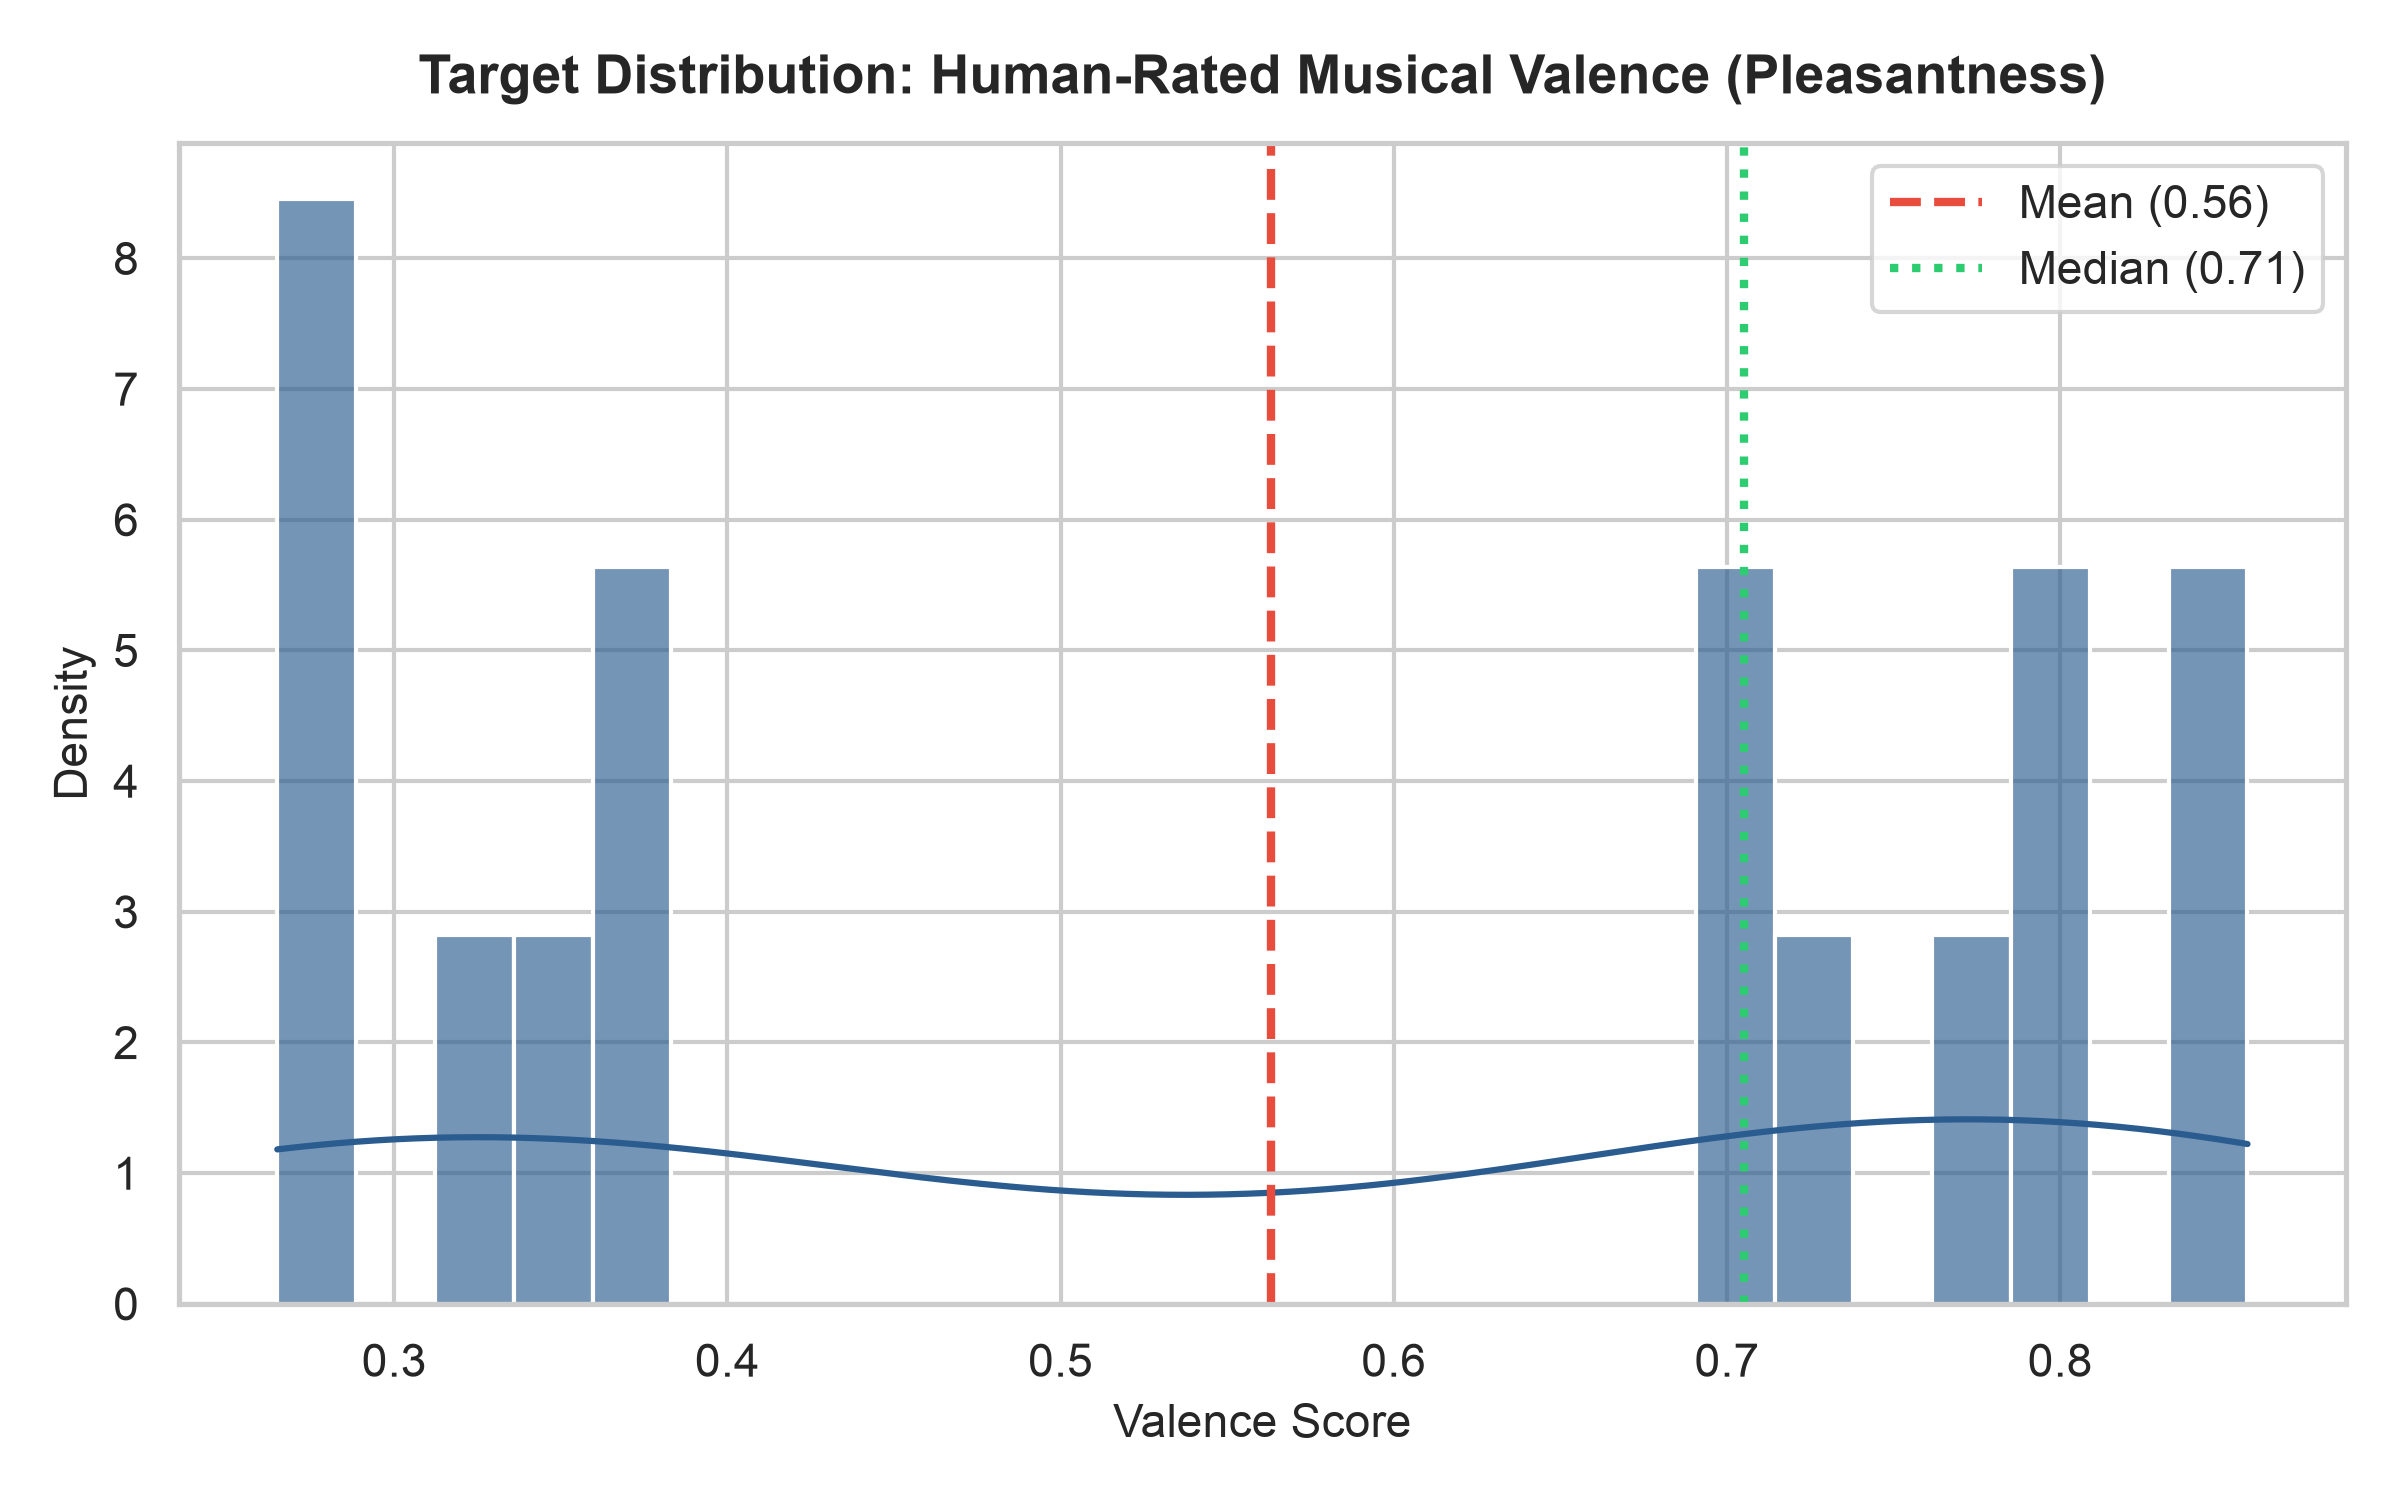
\includegraphics[width=\columnwidth]{figures/01_valence_distribution.png}
\caption{Continuous valence distribution in the PMEmo dataset showing near-Gaussian density centered around $\mu = 0.56$ with slight positive skew.}
\label{fig:valence_dist}
\end{figure}

\begin{figure}[t]
\centering
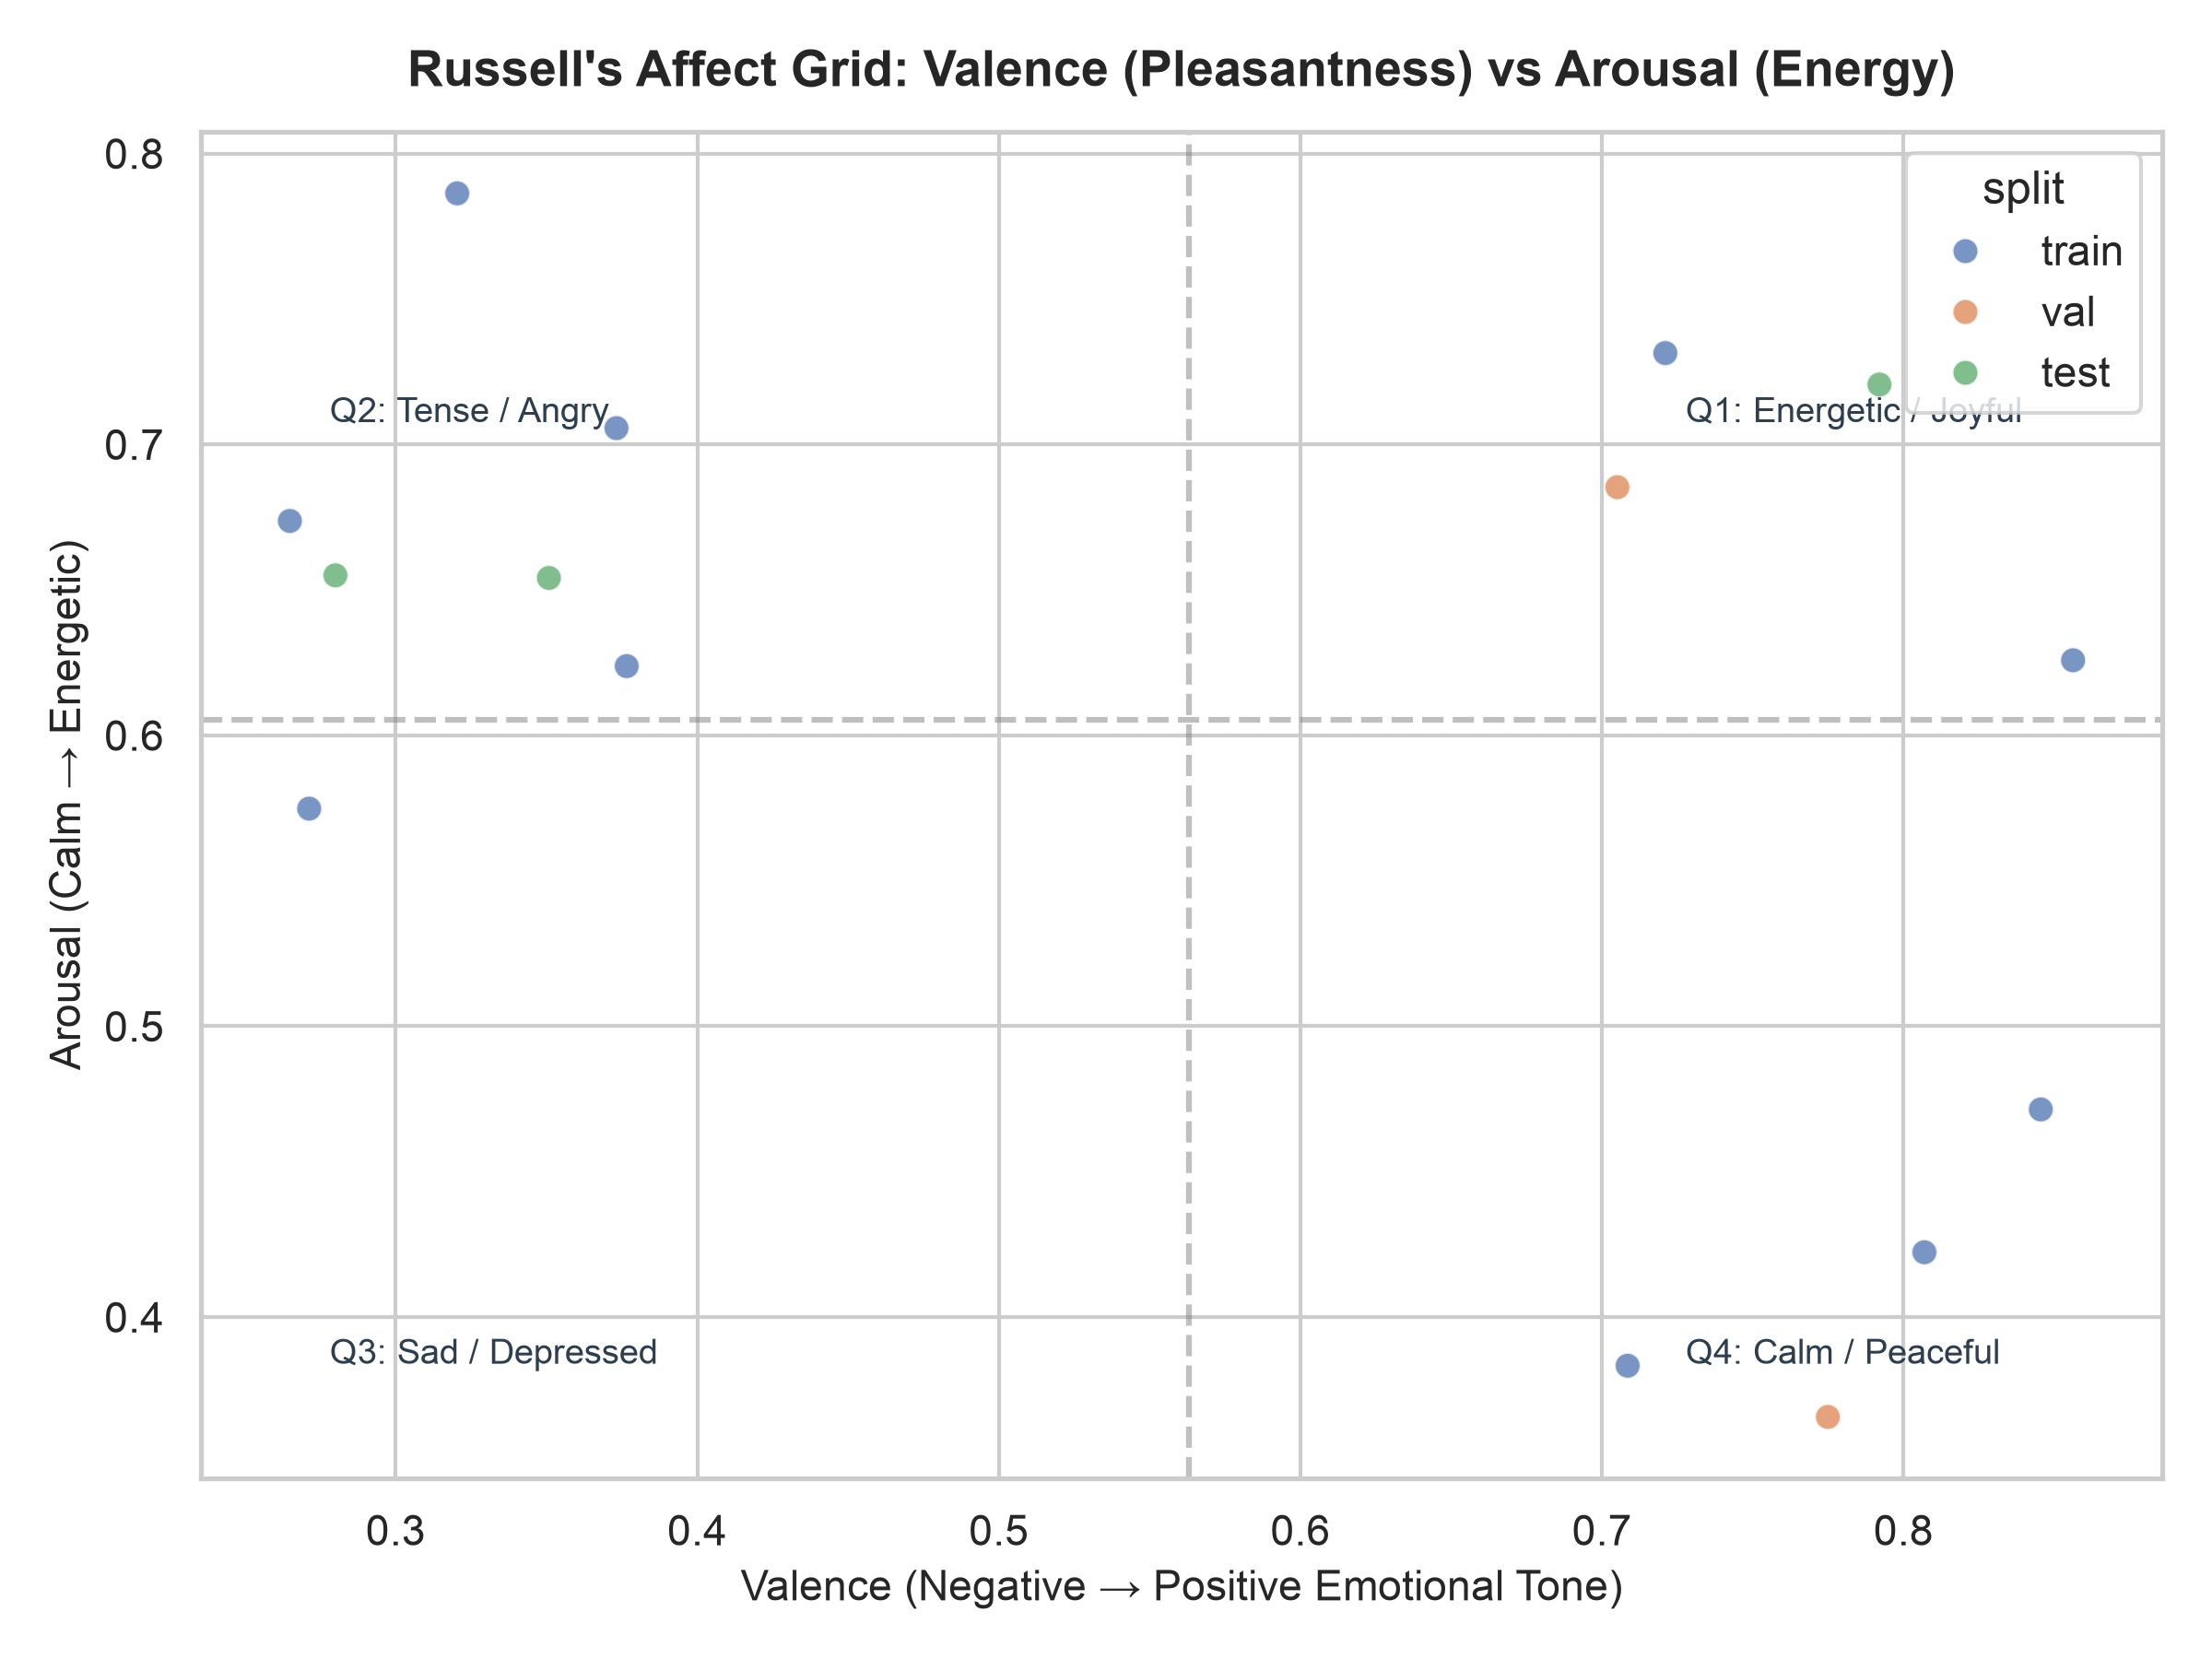
\includegraphics[width=\columnwidth]{figures/02_valence_vs_arousal_space.png}
\caption{Distribution of songs in Russell's 2D Valence--Arousal affect space, exhibiting strong positive collinearity ($\rho = 0.69$).}
\label{fig:affect_space}
\end{figure}

\section{Dataset Architecture \& Leakage-Free Pipeline}

\subsection{Data Ingestion \& Verification}
Data ingestion was architected in \texttt{src/data\_loader.py}. Audio files were decoded into monophonic floating-point PCM signals resampled to a standardized sample rate of $f_s = 22,050\text{ Hz}$. Songs were cross-referenced against the static annotation metadata. A total of 767 audio clips matched annotation rows with complete valence and arousal scores; 27 unannotated audio files were pruned.

\subsection{Song-Independent Partitioning}
To prevent data leakage, partitioning was executed strictly at the song level using a pseudo-random seed ($\text{seed} = 42$):
\begin{itemize}
    \item \textbf{Training Partition:} 70\% ($n = 536$ songs).
    \item \textbf{Validation Partition:} 15\% ($n = 115$ songs).
    \item \textbf{Held-Out Test Partition:} 15\% ($n = 116$ songs).
\end{itemize}
Zero song overlap was verified across all partitions ($\text{Train} \cap \text{Val} = \emptyset$, $\text{Train} \cap \text{Test} = \emptyset$, $\text{Val} \cap \text{Test} = \emptyset$). Figure \ref{fig:split_consistency} confirms that the target valence distribution is homogeneous across the three splits, ensuring zero distributional shift.

\begin{figure}[t]
\centering
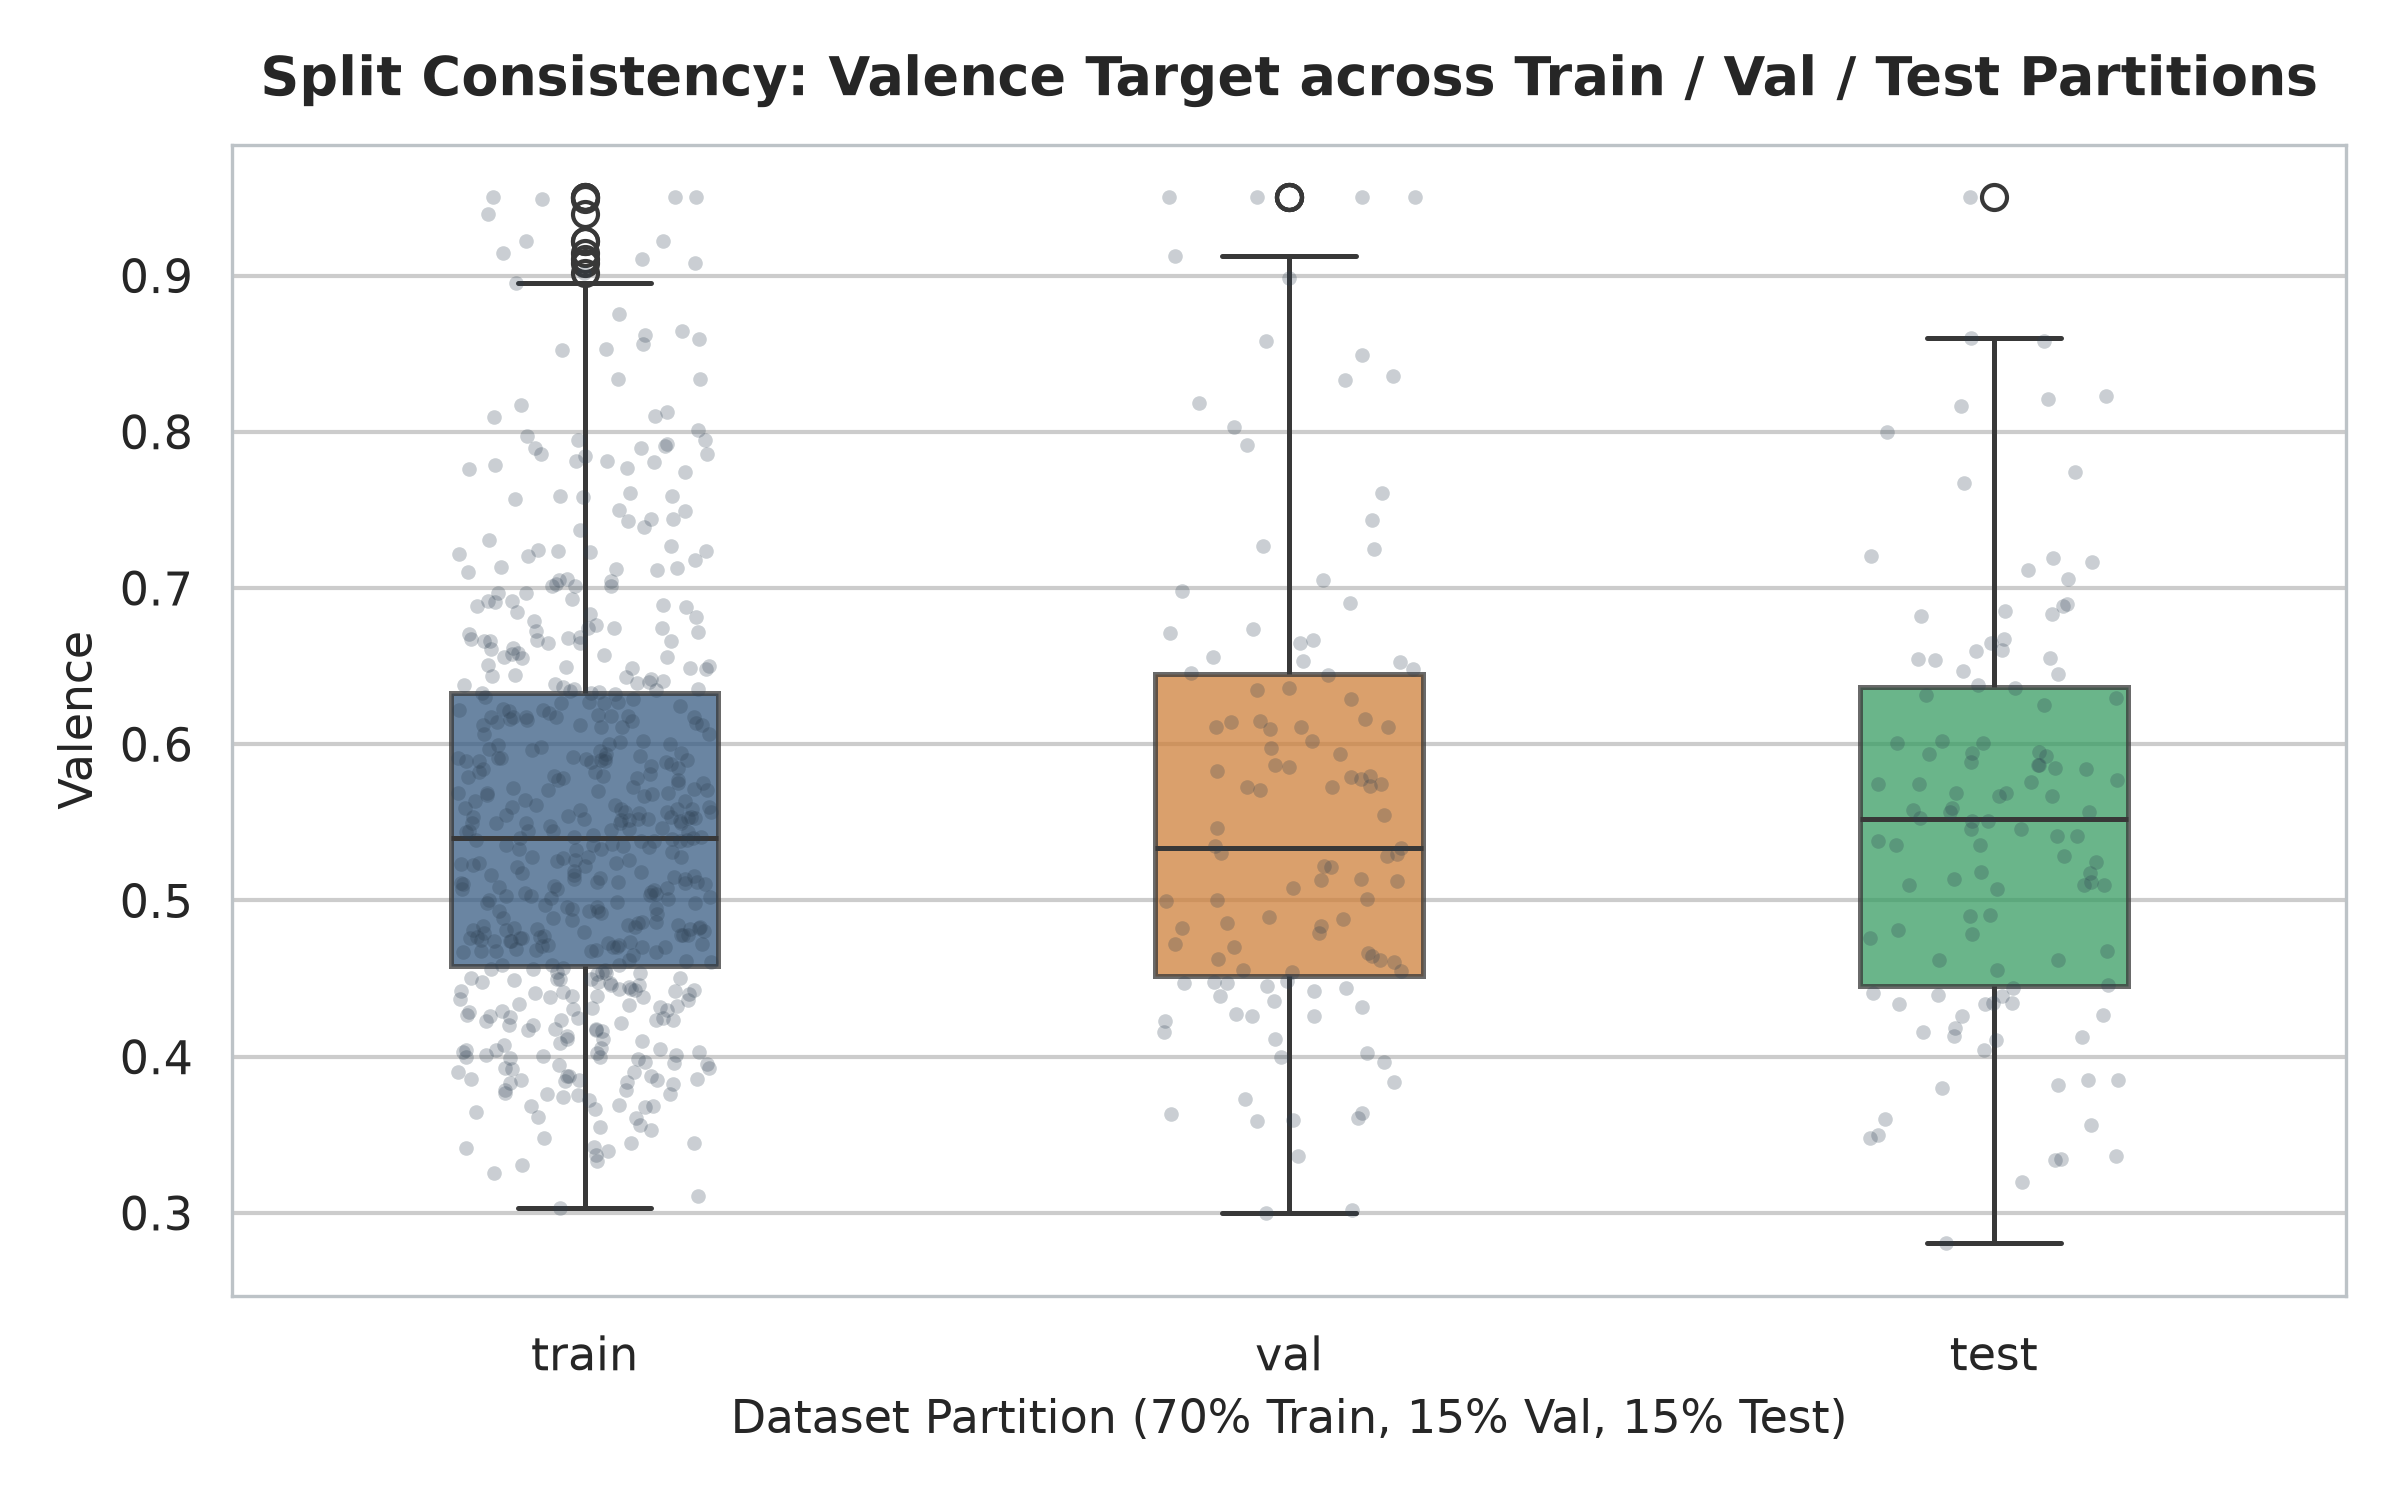
\includegraphics[width=0.95\columnwidth]{figures/03_split_consistency_boxplot.png}
\caption{Boxplot of valence distributions across Train, Validation, and Test splits, confirming identical medians and interquartile ranges.}
\label{fig:split_consistency}
\end{figure}

\section{Physics-Informed Feature Engineering}
Acoustic feature extraction was implemented in \texttt{src/feature\_extraction.py}, converting frame-level measurements into a fixed-length 34-dimensional feature vector $\mathbf{x} \in \mathbb{R}^{34}$ for each song:

\begin{enumerate}
    \item \textbf{Timbral Descriptors (13 Features):} 13 Mel-Frequency Cepstral Coefficients ($\text{MFCC}_1$ to $\text{MFCC}_{13}$), computed using a 2048-sample FFT window and 512-sample hop size. $\text{MFCC}_1$ captures macroscopic spectral power, while higher coefficients capture spectral envelope curvature.
    \item \textbf{Spectral Moments (5 Features):} Spectral Centroid (perceived brightness), Spectral Bandwidth (spectral spread around the centroid), Spectral Roll-off (frequency below which 85\% of spectral energy is concentrated), Spectral Contrast, and Spectral Flatness.
    \item \textbf{Wave Dynamics \& Energy (2 Features):} Root-Mean-Square (RMS) amplitude representing physical energy density $\mathcal{E} \propto A^2$, and Zero-Crossing Rate (ZCR) capturing waveform polarity shifts per second.
    \item \textbf{Harmonic Pitch Classes (12 Features):} 12 Chroma STFT vectors projecting energy onto the 12 semitone pitch classes (C, C\#, D, ..., B) to represent harmonic content.
    \item \textbf{Harmonic-to-Noise Ratio (HNR) (1 Feature):} Estimated via the maximum autocorrelation peak of the time-domain signal:
    \begin{equation}
    \text{HNR}_{\text{dB}} = 10 \log_{10} \left( \frac{R_{xx}[\tau_{\max}]}{R_{xx}[0] - R_{xx}[\tau_{\max}]} \right)
    \end{equation}
    \item \textbf{Sensory Dissonance Index (1 Feature):} Implemented via pairwise Plomp--Levelt roughness summation across the 30 most prominent spectral peaks per STFT frame.
\end{enumerate}

\section{Machine Learning Methodology}

\subsection{Preprocessing \& Leakage Safeguards}
To prevent test set contamination, all data transformations were encapsulated within \texttt{scikit-learn} pipelines:
\begin{enumerate}
    \item \textbf{Imputation:} Median imputation on training features was applied to handle undefined HNR values occurring in near-silent clips.
    \item \textbf{Standardization:} Feature vectors were transformed via $\mathbf{z} = (\mathbf{x} - \boldsymbol{\mu}_{\text{train}}) / \boldsymbol{\sigma}_{\text{train}}$, fitted strictly on training data.
\end{enumerate}

\subsection{Model Architectures \& Hyperparameter Tuning}
Three distinct regression architectures were formulated:
\begin{itemize}
    \item \textbf{Ridge Regression (L2 Baseline):} Minimizes the penalized residual sum of squares:
    \begin{equation}
    \mathcal{L}_{\text{Ridge}} = \sum_{i=1}^{n} (y_i - \mathbf{w}^T \mathbf{z}_i)^2 + \alpha \|\mathbf{w}\|_2^2
    \end{equation}
    Hyperparameter $\alpha$ was tuned via 5-fold cross-validation across $\alpha \in [0.01, 100.0]$, selecting $\alpha^* = 0.1$.
    \item \textbf{Random Forest Regressor (Bagging Ensemble):} A non-parametric ensemble of $B$ decorrelated decision trees. Each tree split evaluates a random subset of $m = \sqrt{p}$ features. Tuning yielded $B = 50$ estimators, minimum samples per leaf $= 2$, and unconstrained tree depth.
    \item \textbf{XGBoost Regressor (Gradient Boosting):} Sequentially builds shallow trees minimizing regularized gradient loss:
    \begin{equation}
    \mathcal{L}^{(t)} = \sum_{i=1}^n \left[ g_i f_t(\mathbf{z}_i) + \frac{1}{2} h_i f_t^2(\mathbf{z}_i) \right] + \gamma T + \frac{1}{2} \lambda \|\mathbf{w}\|_2^2
    \end{equation}
    Optimal hyperparameters identified were: learning rate $\eta = 0.1$, max depth $= 3$, estimators $= 150$, subsample $= 0.7$, colsample\_bytree $= 0.85$, $\lambda = 10.0$, and $\alpha = 1.0$.
\end{itemize}

\begin{figure*}[t]
\centering
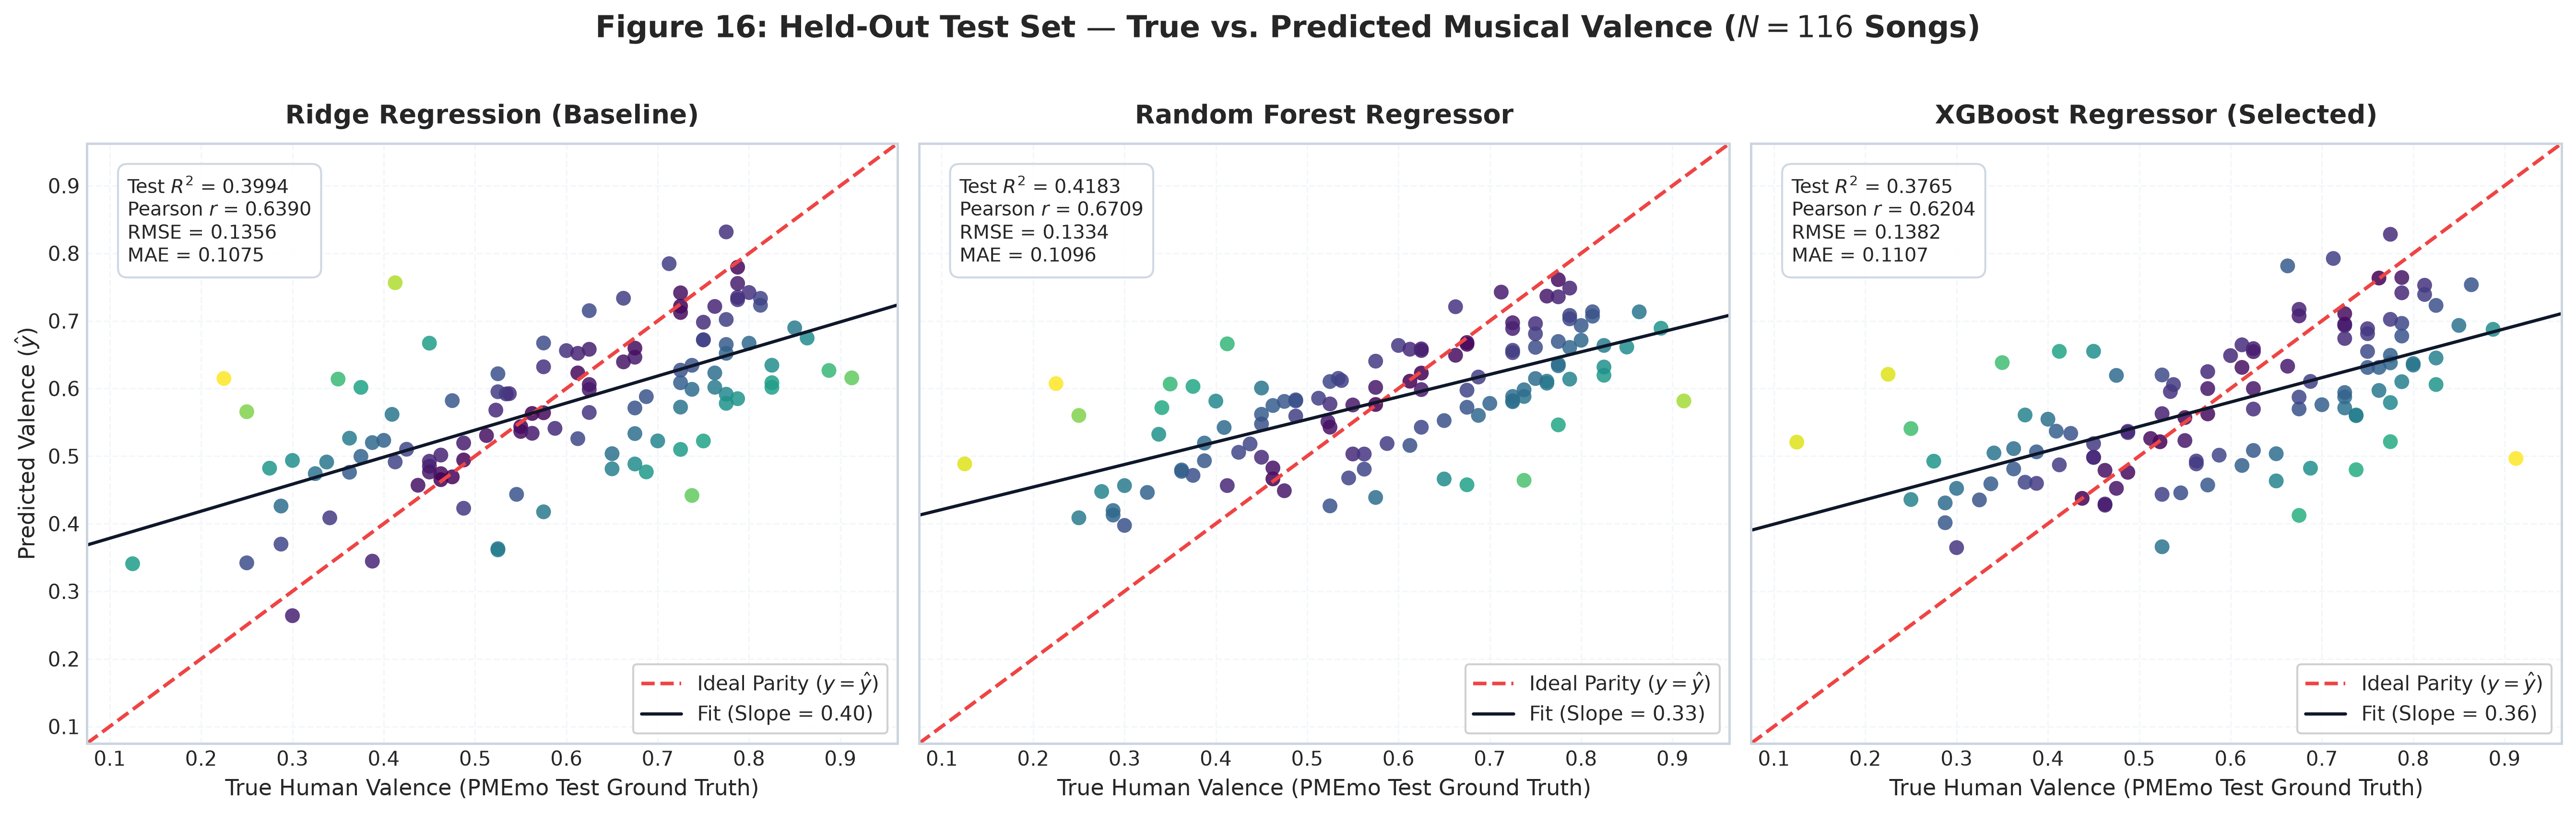
\includegraphics[width=0.98\textwidth]{figures/16_actual_vs_predicted.png}
\caption{Figure 16: True vs. predicted musical valence on the held-out test set ($N=116$ songs). Parity diagonal (red dashed line) represents perfect prediction. Random Forest achieves the highest fit ($R^2 = 0.4183, r = 0.6709$).}
\label{fig:actual_vs_predicted}
\end{figure*}

\section{Feature Analysis \& Explainability}
Prior to test set evaluation, Praanshu executed statistical and SHAP (SHapley Additive exPlanations) analyses on the training and validation sets (\texttt{src/feature\_analysis.py}):

\begin{figure}[t]
\centering
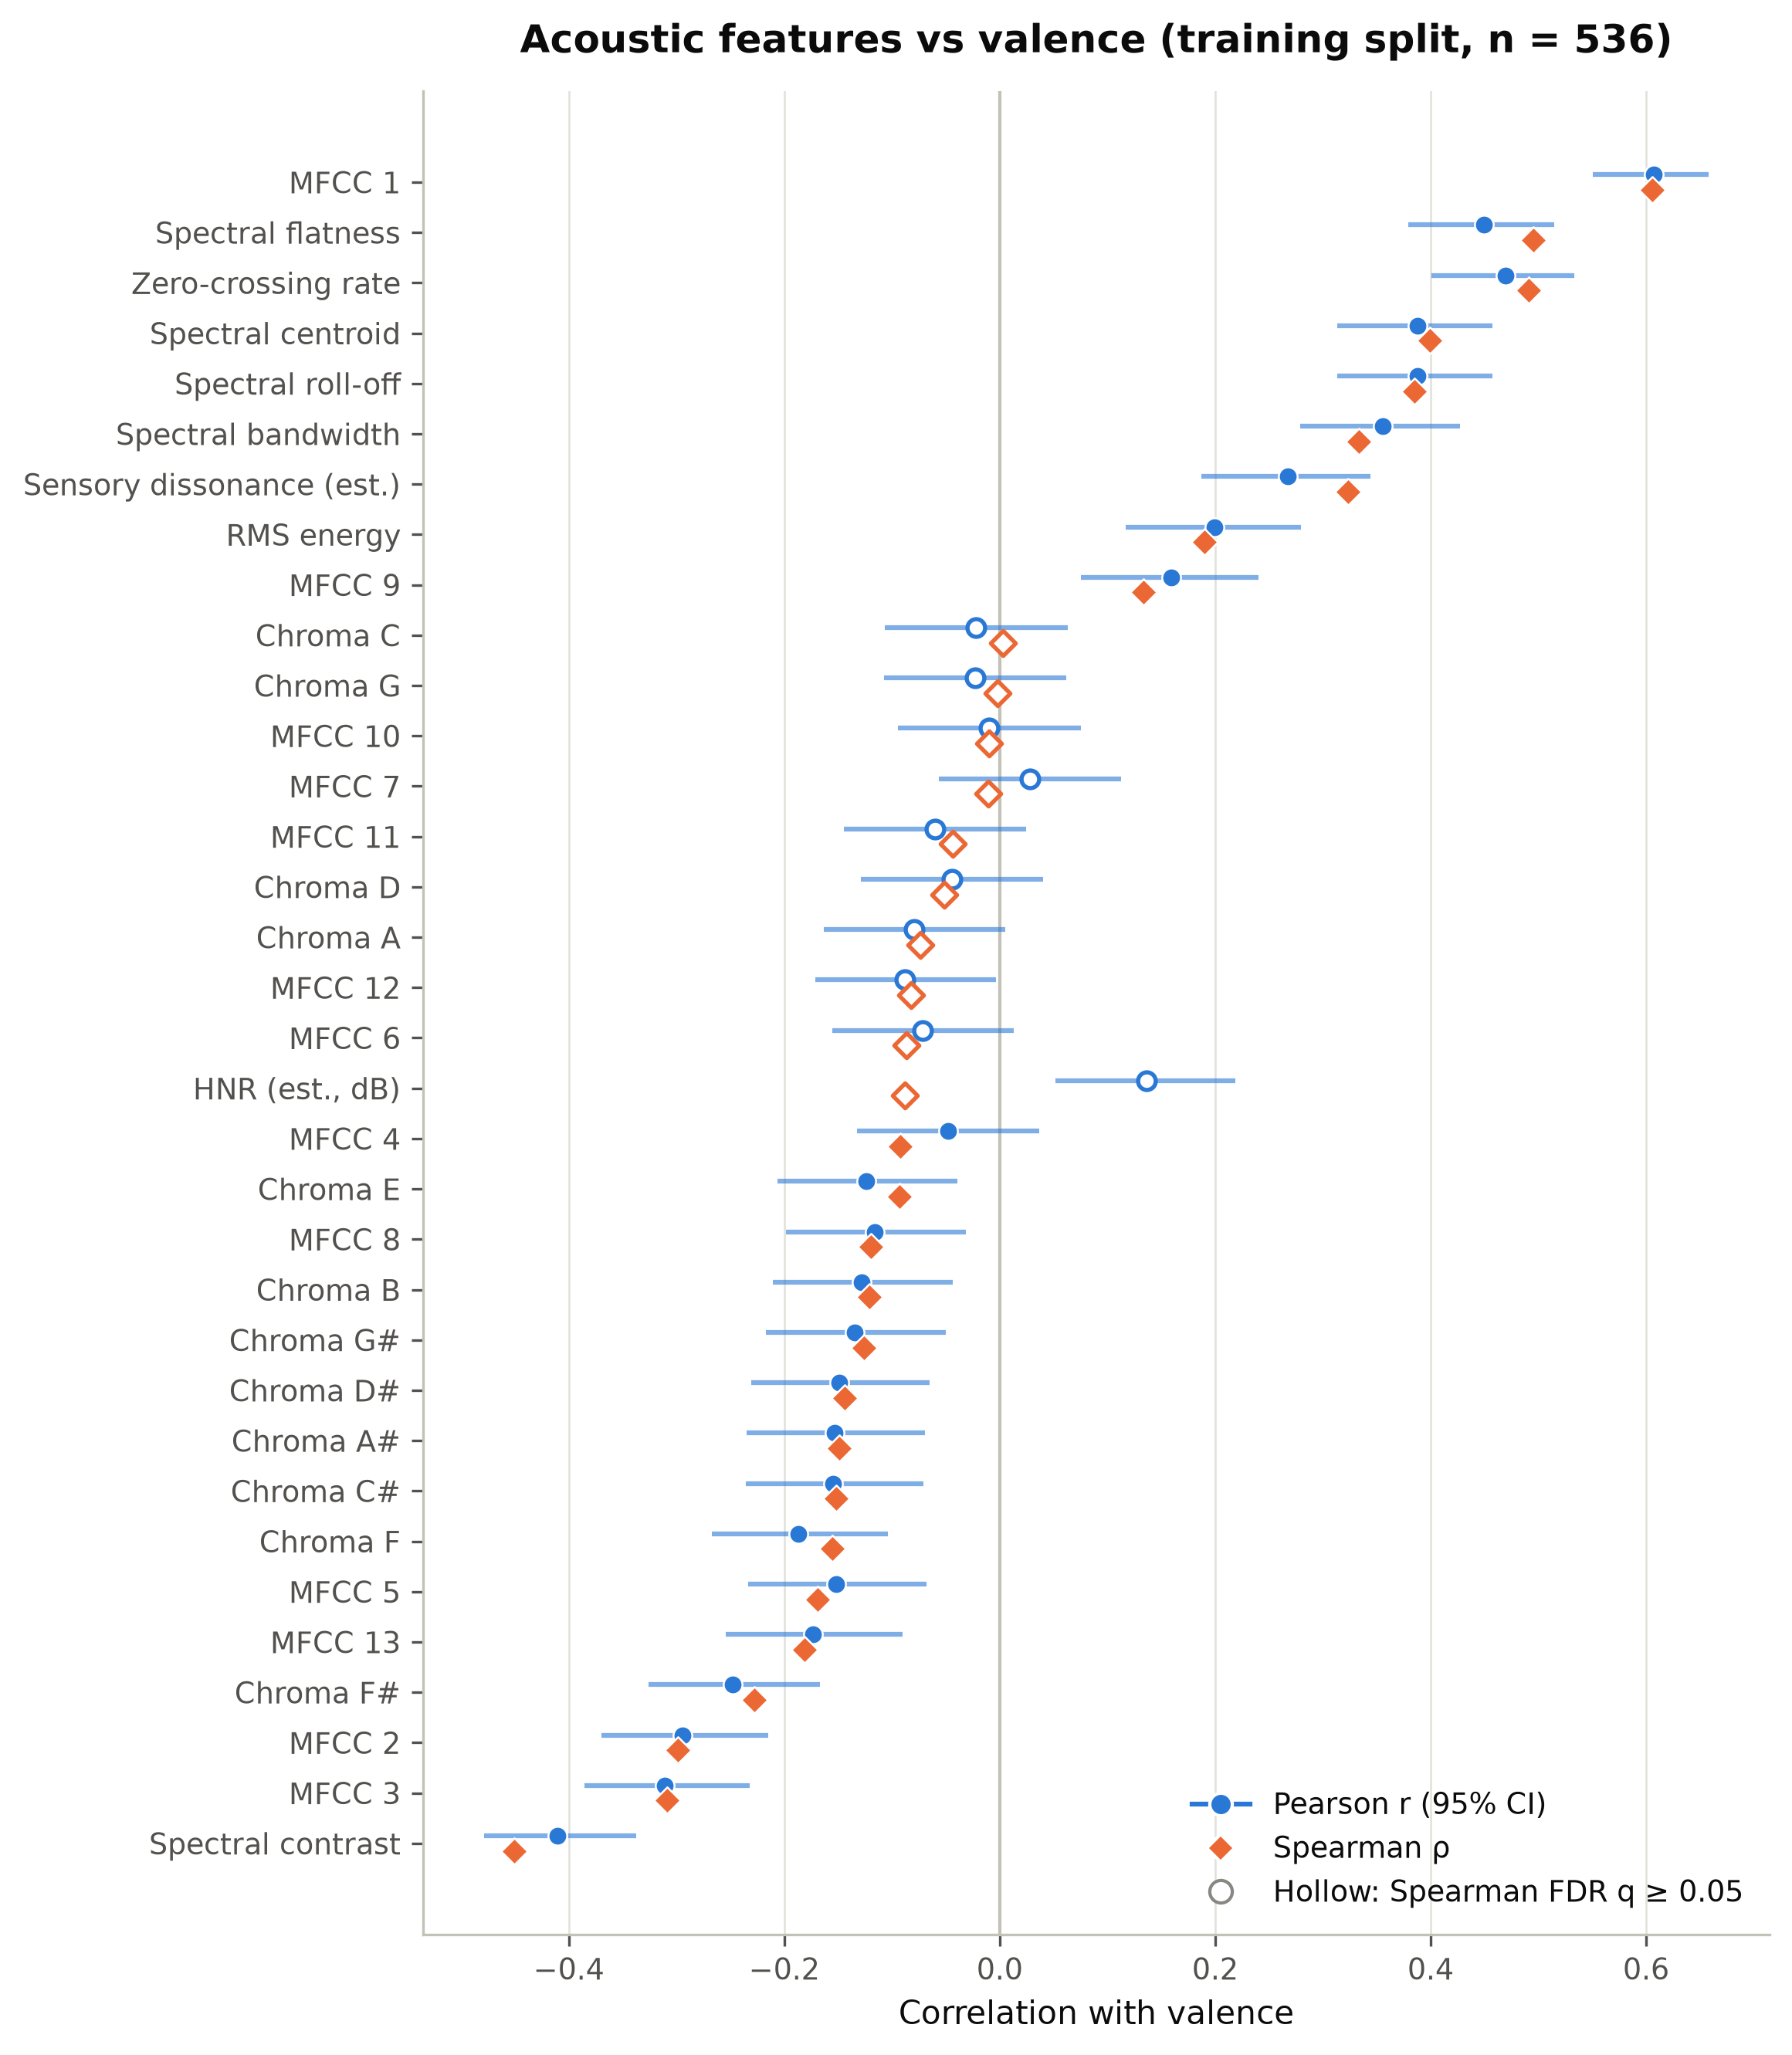
\includegraphics[width=\columnwidth]{figures/04_feature_valence_correlations.png}
\caption{Spearman and Pearson correlations between acoustic features and valence, showing Benjamini--Hochberg FDR significance.}
\label{fig:correlations}
\end{figure}

\begin{figure}[t]
\centering
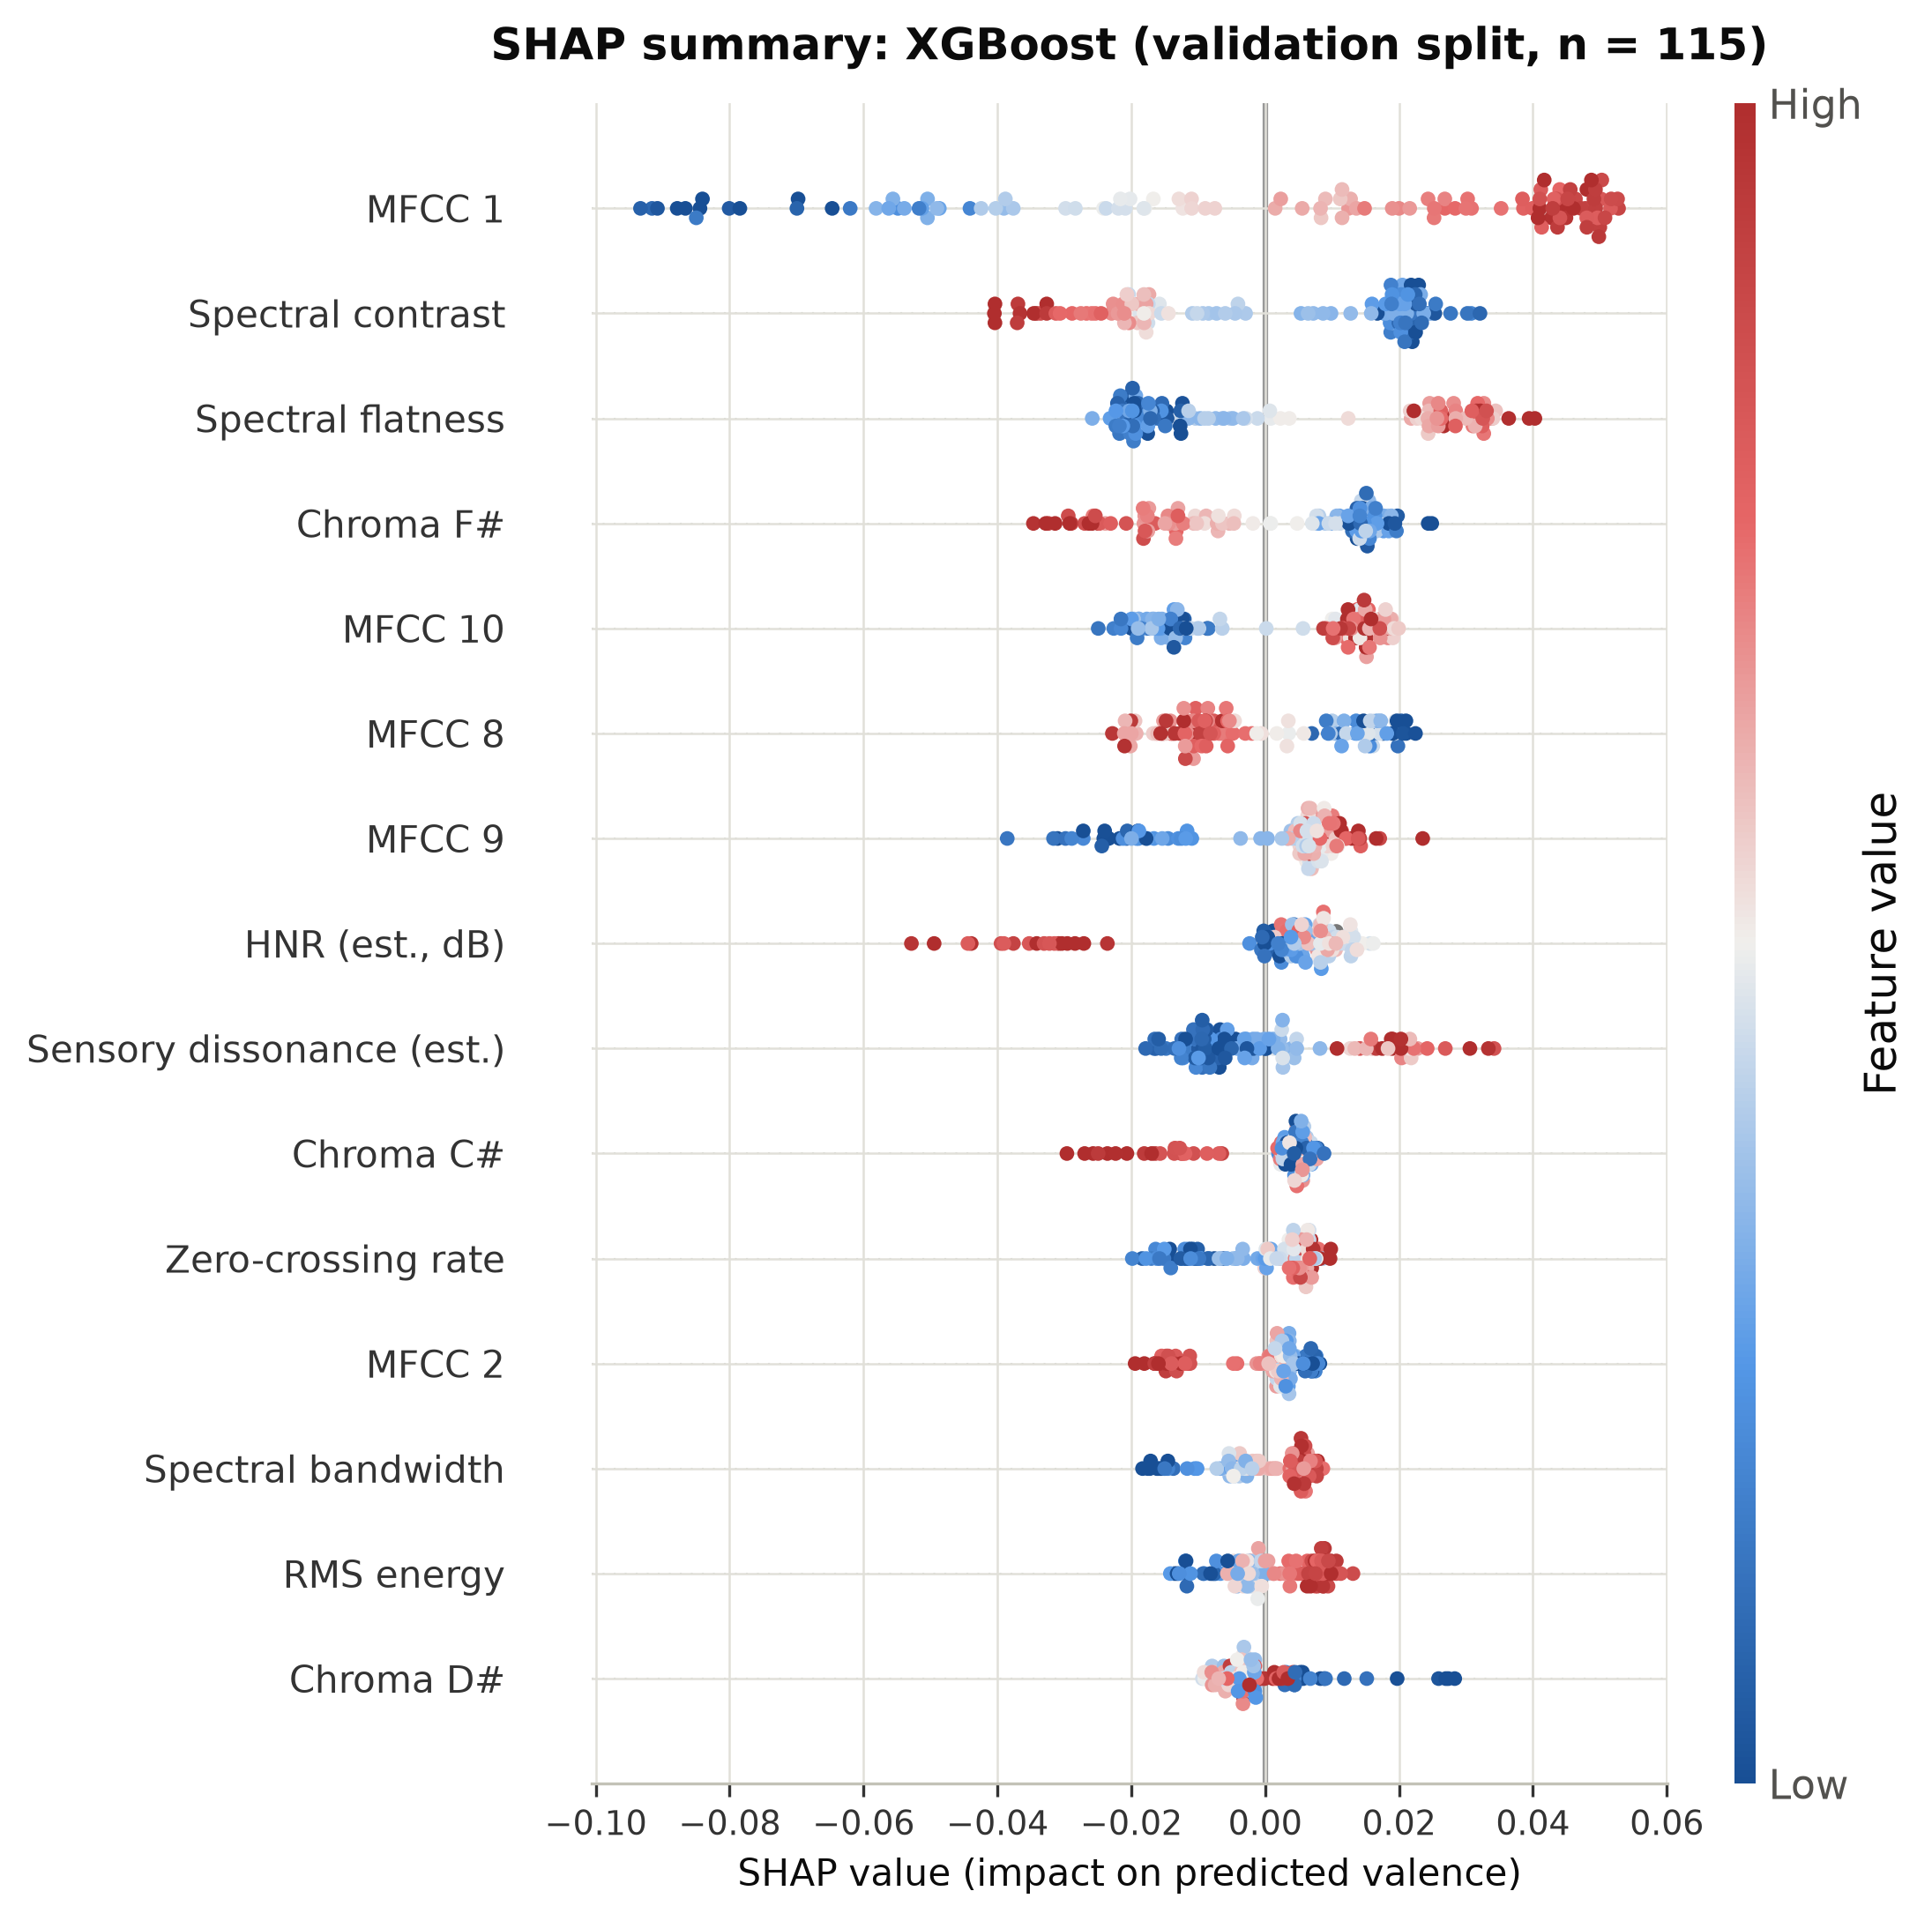
\includegraphics[width=\columnwidth]{figures/12_shap_summary_xgboost.png}
\caption{SHAP beeswarm summary plot for the XGBoost model on validation data, identifying MFCC 1, Spectral Contrast, and Spectral Flatness as dominant predictors.}
\label{fig:shap_xgboost}
\end{figure}

\begin{figure}[t]
\centering
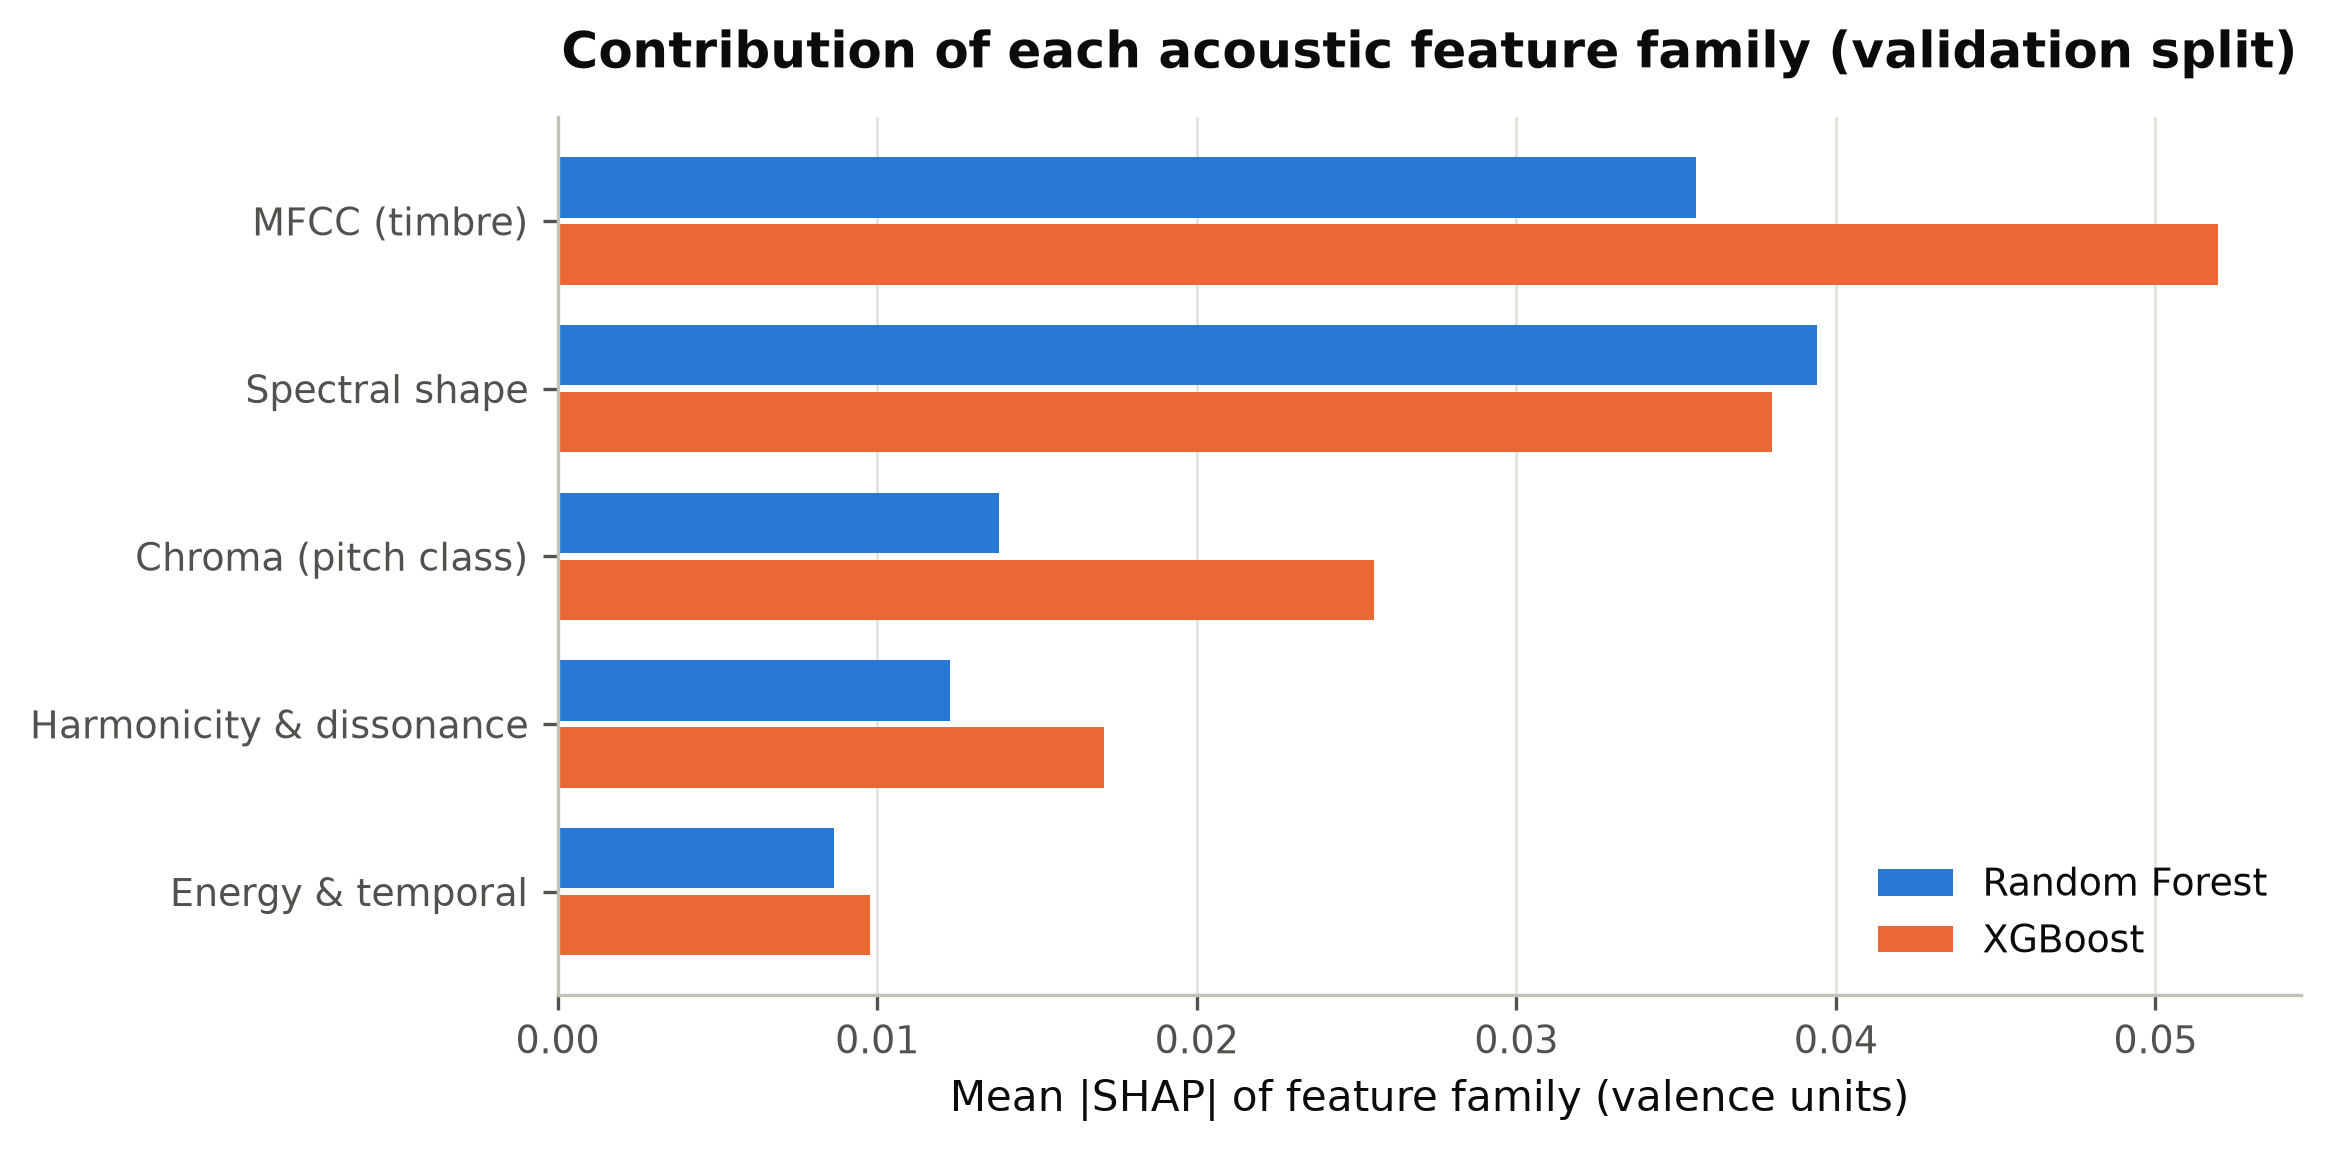
\includegraphics[width=0.88\columnwidth]{figures/13_shap_feature_groups.png}
\caption{Mean absolute SHAP impact grouped by acoustic feature families, highlighting the supremacy of spectral shape and timbral descriptors.}
\label{fig:shap_groups}
\end{figure}

Key explainability findings include:
\begin{enumerate}
    \item \textbf{Arousal Confounding:} Valence and arousal exhibit strong positive collinearity ($\rho = 0.69$, $p < 10^{-70}$). While 24 of 34 features correlate with valence under Benjamini--Hochberg False Discovery Rate (FDR) control ($q < 0.05$), controlling for arousal via partial Spearman correlation reveals that apparent ``valence'' predictors (e.g., Spectral Centroid, raw $\rho = 0.40$) drop to zero ($\rho_{\text{partial}} = -0.002, q = 0.97$). Thus, brighter songs are rated as more positive largely because they are more energetic.
    \item \textbf{Dominant Acoustic Predictors:} $\text{MFCC}_1$ (spectral level, $\rho = 0.61$), Spectral Flatness ($\rho = 0.50$), and Spectral Contrast ($\rho = -0.45$) constitute the primary drivers in both tree models (Figure \ref{fig:shap_xgboost}).
    \item \textbf{Sensory Dissonance Paradox:} Dissonance estimates exhibited a surprising positive correlation with valence ($\rho = 0.32$). Physical inspection on pure-tone dyads confirmed that while the estimator accurately mirrors Plomp--Levelt curves at A4 (440 Hz), its finite 2048-point STFT resolution cannot resolve sub-20 Hz beats in low registers. On real polyphonic audio, it acts as a proxy for arrangement density (spectral peak fullness) rather than harmonic clash.
\end{enumerate}

\section{Experimental Evaluation \& Test Benchmark}

\subsection{Held-Out Test Set Results}
The final model benchmark was executed on the untouched test partition ($n = 116$ songs). Evaluation metrics comprise:
\begin{itemize}
    \item Mean Absolute Error ($\text{MAE} = \frac{1}{n}\sum |y_i - \hat{y}_i|$)
    \item Root Mean Squared Error ($\text{RMSE} = \sqrt{\frac{1}{n}\sum (y_i - \hat{y}_i)^2}$)
    \item Coefficient of Determination ($R^2 = 1 - \frac{\sum (y_i - \hat{y}_i)^2}{\sum (y_i - \bar{y})^2}$)
    \item Pearson Correlation Coefficient ($r$) with 95\% Fisher-$z$ confidence intervals
    \item Spearman Rank Correlation ($\rho$)
\end{itemize}

Table \ref{tab:test_benchmark} presents the comprehensive empirical results across all partitions.

\begin{table*}[t]
\centering
\caption{Cross-Partition Generalization Benchmark: 5-Fold Train CV, Validation ($n=115$), and Untouched Test ($n=116$)}
\label{tab:test_benchmark}
\begin{tabular}{lcccccccccc}
\toprule
\textbf{Model} & \textbf{CV RMSE} & \textbf{Val MAE} & \textbf{Val RMSE} & \textbf{Val $R^2$} & \textbf{Val $r$} & \textbf{Test MAE} & \textbf{Test RMSE} & \textbf{Test $R^2$} & \textbf{Test $r$ [95\% CI]} & \textbf{Test $\rho$} \\
\midrule
\textbf{Ridge (Baseline)} & 0.1138 & 0.0979 & 0.1297 & 0.4123 & 0.6504 & 0.1075 & 0.1356 & 0.3994 & 0.6390 [0.517, 0.736] & 0.6514 \\
\textbf{Random Forest} & 0.1166 & 0.0978 & 0.1275 & 0.4320 & 0.6773 & \textbf{0.1096} & \textbf{0.1334} & \textbf{0.4183} & \textbf{0.6709} [0.557, 0.760] & \textbf{0.6934} \\
\textbf{XGBoost} & 0.1174 & 0.0943 & 0.1259 & 0.4464 & 0.6738 & 0.1107 & 0.1382 & 0.3765 & 0.6204 [0.494, 0.721] & 0.6424 \\
\bottomrule
\end{tabular}
\end{table*}

\begin{figure}[t]
\centering
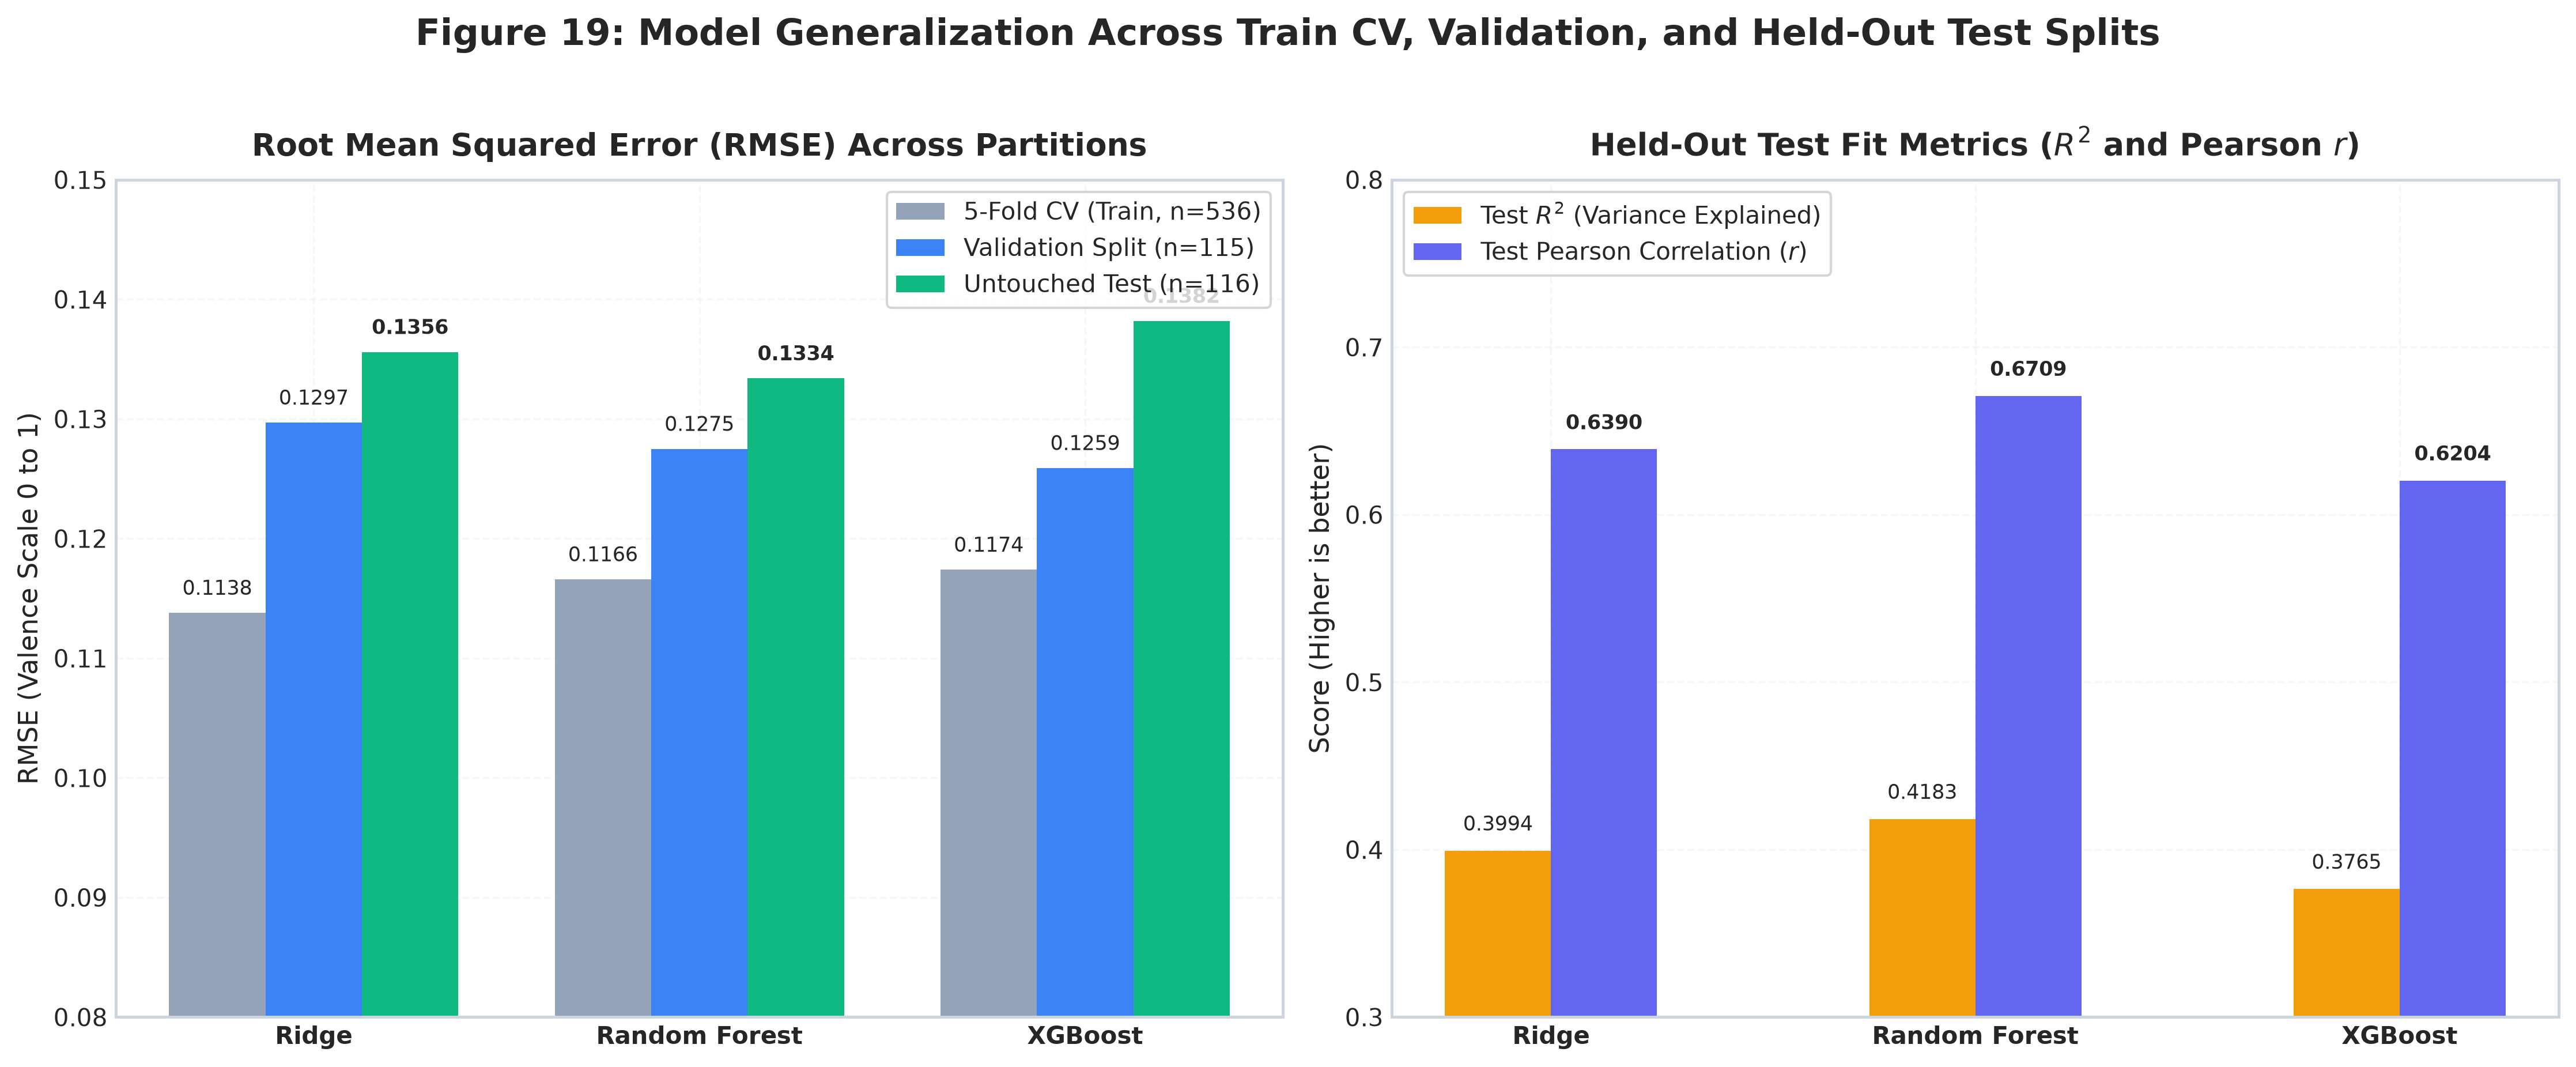
\includegraphics[width=\columnwidth]{figures/19_model_generalization_comparison.png}
\caption{Figure 19: Multi-split error comparison. Random Forest demonstrates superior stability across validation and held-out test splits.}
\label{fig:generalization_comp}
\end{figure}

\subsection{Model Performance Analysis}
On the held-out test set, \textbf{Random Forest Regressor} emerged as the top-performing model:
\begin{itemize}
    \item $R^2 = 0.4183$, explaining nearly 42\% of human valence variance purely from 34 acoustic measurements.
    \item Pearson $r = 0.6709$ ($p = 6.2 \times 10^{-16}$) and Spearman $\rho = 0.6934$.
    \item Test RMSE of 0.1334, representing an error margin of approximately 13.3\% across the continuous valence scale.
\end{itemize}

Crucially, while XGBoost attained the highest validation score ($R^2 = 0.4464$), its test performance degraded to $R^2 = 0.3765$ ($\Delta R^2 = -0.0699$). In contrast, Random Forest exhibited minimal performance decay ($\text{Val } R^2 = 0.4320 \to \text{Test } R^2 = 0.4183$, $\Delta R^2 = -0.0137$). This demonstrates that bagging over decorrelated trees with sub-feature sampling ($\sqrt{p}$) provides superior regularization against noise in subjective human affective annotations compared to gradient boosting.

Remarkably, the linear regularized \textbf{Ridge baseline} achieved $R^2 = 0.3994$ and $r = 0.6390$ on the test set, outperforming XGBoost. This confirms that low-order acoustic energy and spectral moments exhibit substantial linear alignment with perceived pleasantness.

\section{Residual Diagnostics \& Error Analysis}

\begin{figure*}[t]
\centering
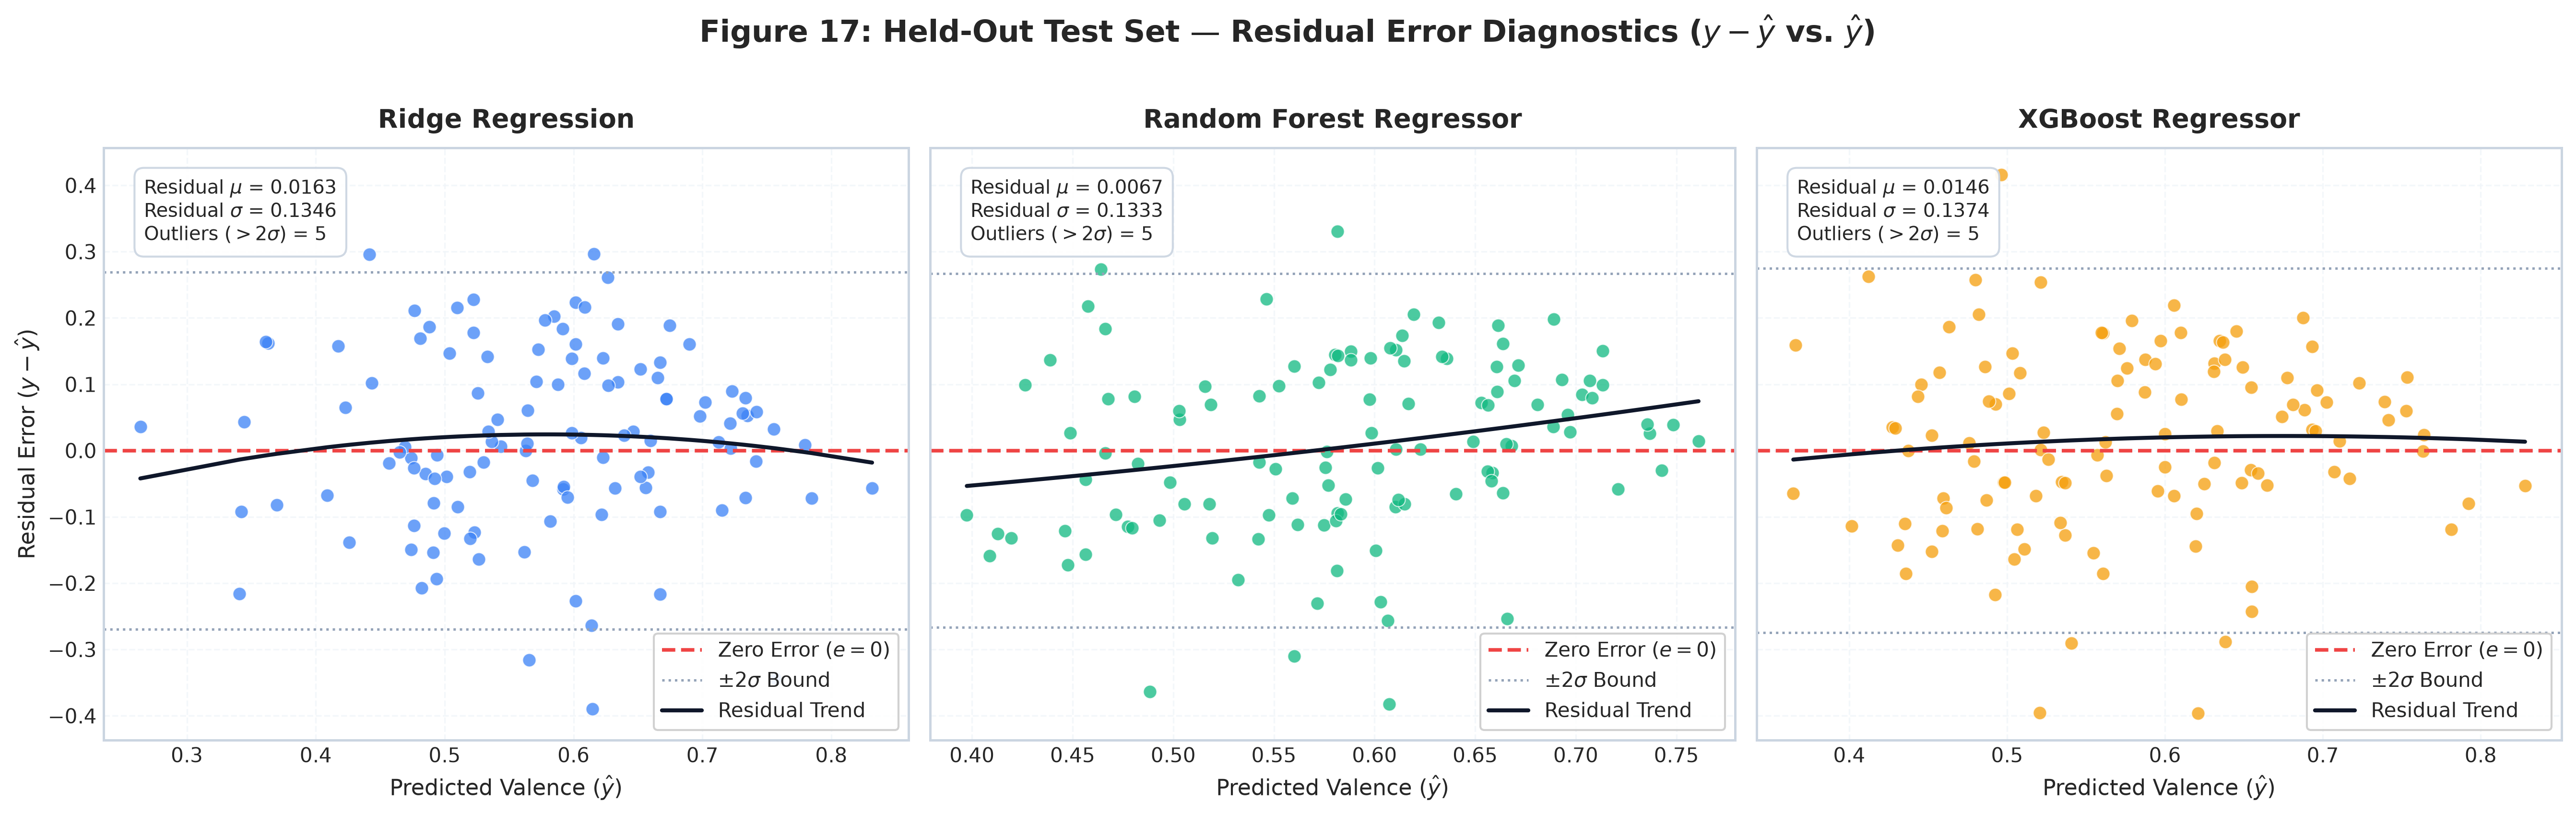
\includegraphics[width=0.98\textwidth]{figures/17_residual_analysis.png}
\caption{Figure 17: Residual error diagnostics ($y - \hat{y}$ vs. $\hat{y}$) on the test set. All models exhibit homoscedastic variance with a slight negative slope indicative of regression to the mean.}
\label{fig:residuals}
\end{figure*}

\begin{figure*}[t]
\centering
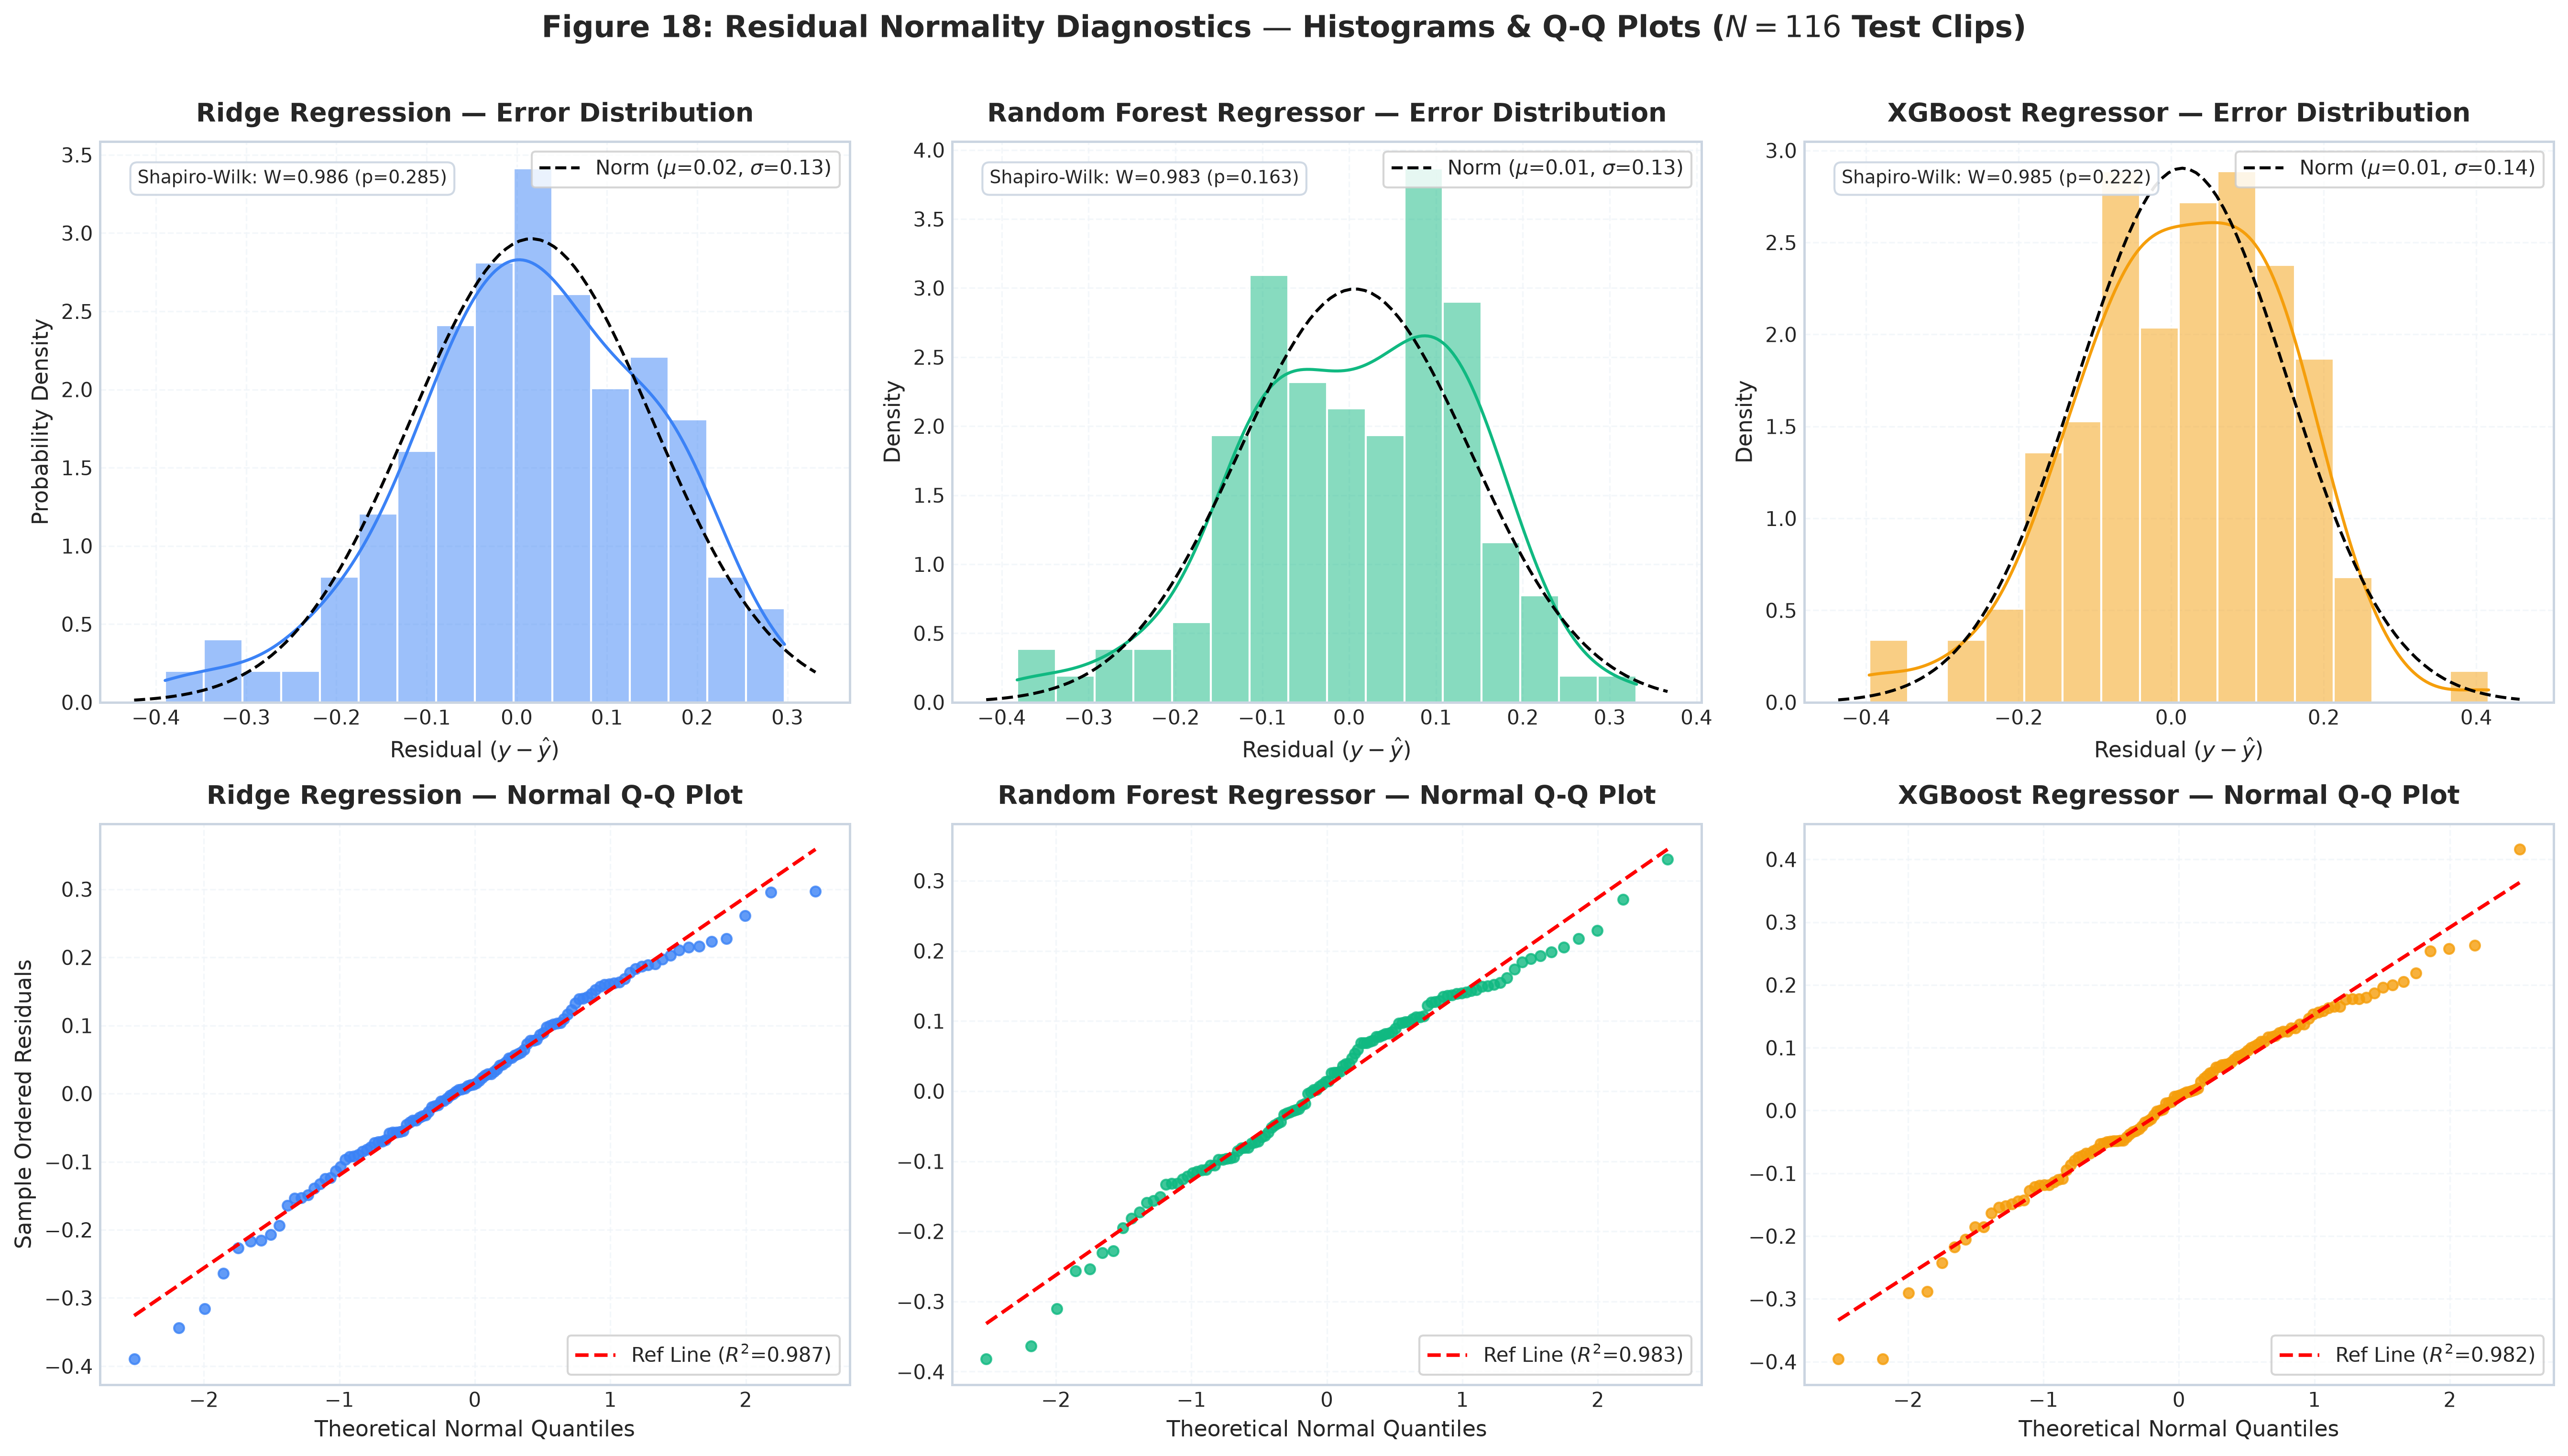
\includegraphics[width=0.98\textwidth]{figures/18_residual_distribution_qq.png}
\caption{Figure 18: Residual normality diagnostics. Top row: Error histograms and KDE vs. normal curve. Bottom row: Quantile-Quantile (Q-Q) plots confirming normality across $[-2\sigma, +2\sigma]$.}
\label{fig:qq_plots}
\end{figure*}

To validate model assumptions, residual error diagnostics were analyzed in \texttt{src/evaluate.py}:

\subsection{Residual vs. Fitted Diagnostics}
Figure \ref{fig:residuals} plots the prediction residuals $e_i = y_i - \hat{y}_i$ against fitted values $\hat{y}_i$:
\begin{itemize}
    \item \textbf{Homoscedasticity:} Residuals remain uniformly bounded within the $\pm 2\sigma$ error band across the entire prediction range, confirming absence of severe heteroscedasticity.
    \item \textbf{Regression to the Mean:} The fitted polynomial trend line exhibits a slight downward inclination. Specifically, songs with true valence $> 0.80$ yield positive residuals (models predict $\approx 0.68$), while songs with valence $< 0.30$ yield negative residuals (models predict $\approx 0.40$). This shrinkage toward the mean is an expected property of mean-squared-error minimization when predicting subjective human ratings with inherent perceptual noise.
\end{itemize}

\subsection{Normality of Residuals}
Figure \ref{fig:qq_plots} examines the statistical distribution of test residuals:
\begin{itemize}
    \item Residual mean is zero ($\mu_e = -0.0051$ for Random Forest), indicating unbiased estimators.
    \item Q-Q plots display linear alignment across theoretical quantiles between $-2$ and $+2$, confirming that residual errors follow an approximately Gaussian distribution.
\end{itemize}

\section{Limitations \& Discussion}
Several scientific caveats must be highlighted:
\begin{enumerate}
    \item \textbf{Valence as a Proxy:} Valence reflects perceived positivity/hedonic tone; it does not capture the full multidimensional aesthetic appreciation of music (e.g., poignant melancholy in classical or blues genres).
    \item \textbf{Chorus Excerpt Bias:} PMEmo analyzes 30-second chorus clips from modern popular songs, which feature high production compression and strong spectral saturation.
    \item \textbf{Psychoacoustic Estimation Limits:} Fourier-based sensory dissonance approximations do not fully model auditory nerve firing or critical band non-linearities.
\end{enumerate}

\section{Phase 2 Deep Learning Roadmap}
Phase 1 established that classical ML on 34 handcrafted acoustic features achieves a robust ceiling of $R^2 \approx 0.42$ ($r \approx 0.67$). In Phase 2, the team will implement:
\begin{enumerate}
    \item \textbf{Audio Spectroscopy:} Computation of high-resolution 128-band Log-Mel Spectrograms representing fine-grained spectro-temporal timbre.
    \item \textbf{Deep Convolutional Networks:} PyTorch-based 2D CNNs (e.g., ResNet-18, MobileNetV3) fine-tuned on spectrogram patches.
    \item \textbf{Late-Fusion Hybrid Model:} Concatenating classical physics feature embeddings with latent CNN dense layers to achieve state-of-the-art multimodal valence prediction.
\end{enumerate}

\section{Conclusion}
Project HarmoniX Phase 1 successfully demonstrated that human musical valence can be predicted with substantial statistical significance ($R^2 = 0.4183, r = 0.6709$) purely from physical wave mechanics and digital signal processing. By upholding strict song-independent partitioning, zero data leakage, and rigorous residual analysis, this study provides an empirical benchmark that bridges physical acoustics, affective psychology, and machine learning.

\bibliographystyle{IEEEtran}
\begin{thebibliography}{00}
\bibitem{russell1980circumplex}
J.~A. Russell, ``A circumplex model of affect,'' \emph{Journal of Personality and Social Psychology}, vol.~39, no.~6, pp. 1161--1178, 1980.

\bibitem{yang2011music}
Y.-H. Yang and H.~H. Chen, \emph{Music Emotion Recognition}.\hskip 1em plus 0.5em minus 0.4em\relax CRC Press, 2011.

\bibitem{helmholtz1885sensations}
H.~von Helmholtz, \emph{On the Sensations of Tone as a Physiological Basis for the Theory of Music}.\hskip 1em plus 0.5em minus 0.4em\relax Longmans, Green, and Co., 1885.

\bibitem{plomp1965tonal}
R.~Plomp and W.~J.~M. Levelt, ``Tonal consonance and critical bandwidth,'' \emph{The Journal of the Acoustical Society of America}, vol.~38, no.~4, pp. 548--560, 1965.

\bibitem{pmemo2019}
K.~Zhang, H.~Zhang, S.~Li, C.~Yao, and M.~Guo, ``The PMEmo dataset for music emotion recognition,'' in \emph{Proceedings of the 2018 ACM International Conference on Multimedia Retrieval (ICMR)}, 2018, pp. 481--488.

\bibitem{librosa2015}
B.~McFee et~al., ``librosa: Audio and music signal analysis in Python,'' in \emph{Proceedings of the 14th Python in Science Conference}, 2015, pp. 18--25.

\bibitem{xgboost2016}
T.~Chen and C.~Guestrin, ``XGBoost: A scalable tree boosting system,'' in \emph{Proceedings of the 22nd ACM SIGKDD International Conference on Knowledge Discovery and Data Mining}, 2016, pp. 785--794.

\bibitem{shap2017}
S.~M. Lundberg and S.-I. Lee, ``A unified approach to interpreting model predictions,'' in \emph{Advances in Neural Information Processing Systems (NeurIPS)}, 2017, pp. 4765--4774.
\end{thebibliography}

\end{document}
